\documentclass[11pt,a4paper]{article}

\usepackage[utf8]{inputenc}
\usepackage[T1]{fontenc}
\usepackage[spanish,es-nodecimaldot]{babel}
\usepackage{amsmath}
\usepackage{booktabs}
\usepackage{tabularx}
\usepackage{array}
\usepackage{graphicx}
\usepackage{geometry}
\usepackage{xcolor}
\usepackage{float}
\usepackage{caption}
\usepackage{hyperref}
\geometry{margin=2.2cm}

\hypersetup{
    colorlinks=true,
    linkcolor=blue!50!black,
    urlcolor=blue!50!black,
    pdftitle={Reporte comparativo de corridas largas base y residual},
    pdfauthor={Cesar Zapata}
}

\newcolumntype{Y}{>{\raggedright\arraybackslash}X}

\title{Reporte comparativo de corridas largas sobre \texttt{Agent7250} y sobre la l\'inea residual\\\large Proyecto TD3 para pr\'otesis mioel\'ectrica}
\author{C\'esar Zapata\\Research Laboratory in Artificial Intelligence and Computer Vision ``Alan Turing''}
\date{4 de abril de 2026}

\begin{document}
\maketitle

\section*{Prop\'osito real de estas dos corridas largas}
Este documento compara las dos corridas de 50000 episodios ejecutadas despu\'es de cerrar la primera fase fuerte del proyecto:
\begin{itemize}
    \item una corrida larga base que continu\'o \texttt{Agent7250} como TD3 plano;
    \item una corrida larga residual que continu\'o la l\'inea \texttt{Residual Lift} sobre \texttt{Agent7250}.
\end{itemize}

Es importante fijar desde el inicio la pregunta correcta. Estas corridas \textbf{no se lanzaron principalmente para forzar una mejora del agente}, sino para observar qu\'e pasa cuando el entrenamiento se extiende mucho m\'as all\'a de las corridas normales:
\begin{enumerate}
    \item si aparece una mejora sostenida;
    \item si el agente entra en meseta;
    \item o si comienza a desaprender y deriva hacia un compromiso peor.
\end{enumerate}

Por eso, el valor de estas corridas largas no est\'a solo en su mejor checkpoint, sino en lo que revelan sobre la \textbf{evoluci\'on temporal} del entrenamiento.

\section*{Punto de partida antes de las corridas largas}
Antes de estas dos extensiones a 50000 episodios, el estado del proyecto era el siguiente:
\begin{itemize}
    \item \textbf{Benchmark oficial estable:} \texttt{Agent7250}.
    \item \textbf{Mejor residual reproducible:} la \texttt{seed 22}, aceptada bajo \texttt{ConditionA}.
    \item \textbf{Mejor residual single-run hist\'orico:} \texttt{Agent1850}, aceptado bajo \texttt{ConditionB} y todav\'ia el mejor compromiso hist\'orico entre tracking, esfuerzo y saturaci\'on.
\end{itemize}

En consecuencia, ninguna de las corridas largas se interpret\'o como reemplazo autom\'atico del benchmark. Las dos se plantearon como \textbf{experimentos exploratorios de horizonte temporal}.

\section*{Corrida larga base sobre \texttt{Agent7250}}
\subsection*{Configuraci\'on}
La corrida base continu\'o el checkpoint can\'onico \texttt{Agent7250} como TD3 plano, sin residual, manteniendo la observaci\'on \texttt{markov52}, la reward validada y guardado espaciado de checkpoints.

\begin{table}[H]
\centering
\caption{Configuraci\'on principal de la corrida larga base}
\begin{tabularx}{\linewidth}{lY}
\toprule
Elemento & Valor \\
\midrule
Carpeta experimental & \texttt{Agentes/agen\_7250\_Corrida\_larga} \\
Agente & \texttt{td3} \\
Checkpoint de arranque & \texttt{Agent7250} \\
Episodios de entrenamiento & 50000 \\
Guardado de checkpoints & cada 500 episodios \\
Guardado de episodios & cada 500 episodios \\
Plots de entrenamiento & \texttt{none} \\
Semilla controlada & no (\texttt{randomSeed = NaN}) \\
\bottomrule
\end{tabularx}
\end{table}

\subsection*{Curva de entrenamiento}
\begin{figure}[H]
\centering
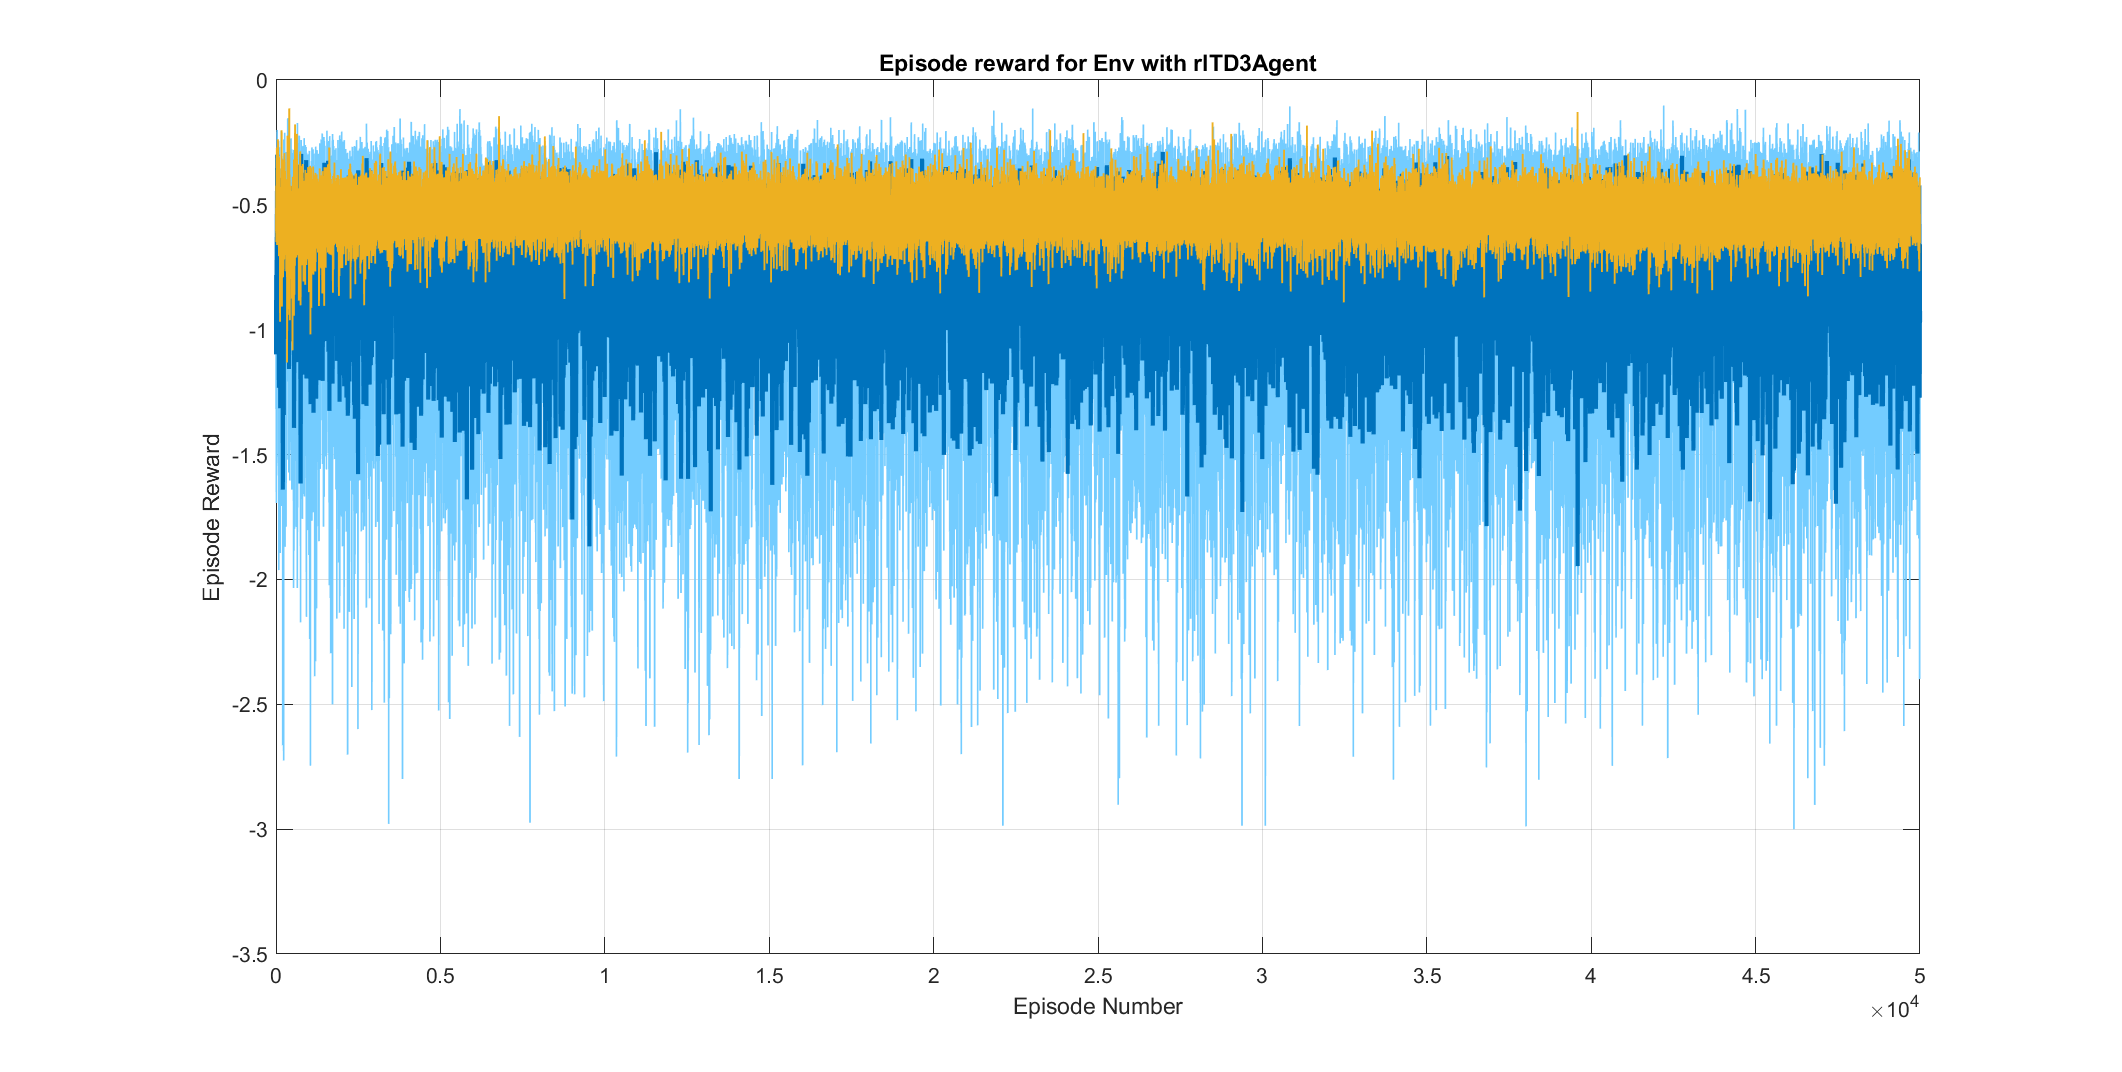
\includegraphics[width=\linewidth]{figures/agent7250_longrun_training_progress_20260404.png}
\caption{Curva de entrenamiento de la corrida larga base sobre \texttt{Agent7250}.}
\label{fig:base_training}
\end{figure}

La lectura principal de esta curva es:
\begin{itemize}
    \item episodios totales: 50000;
    \item mejor \texttt{AverageReward}: \(-0.287762\) en el episodio 26969;
    \item \texttt{AverageReward} final: \(-0.970405\).
\end{itemize}

Esto indica que la mejor zona de la corrida apareci\'o bastante antes del final. En vez de consolidar una mejora sostenida hasta el episodio 50000, el entrenamiento termin\'o con un promedio claramente peor, lo que es consistente con \textbf{deriva tard\'ia} o desaprendizaje parcial.

\subsection*{Auditor\'ia de toda la trayectoria}
\begin{figure}[H]
\centering
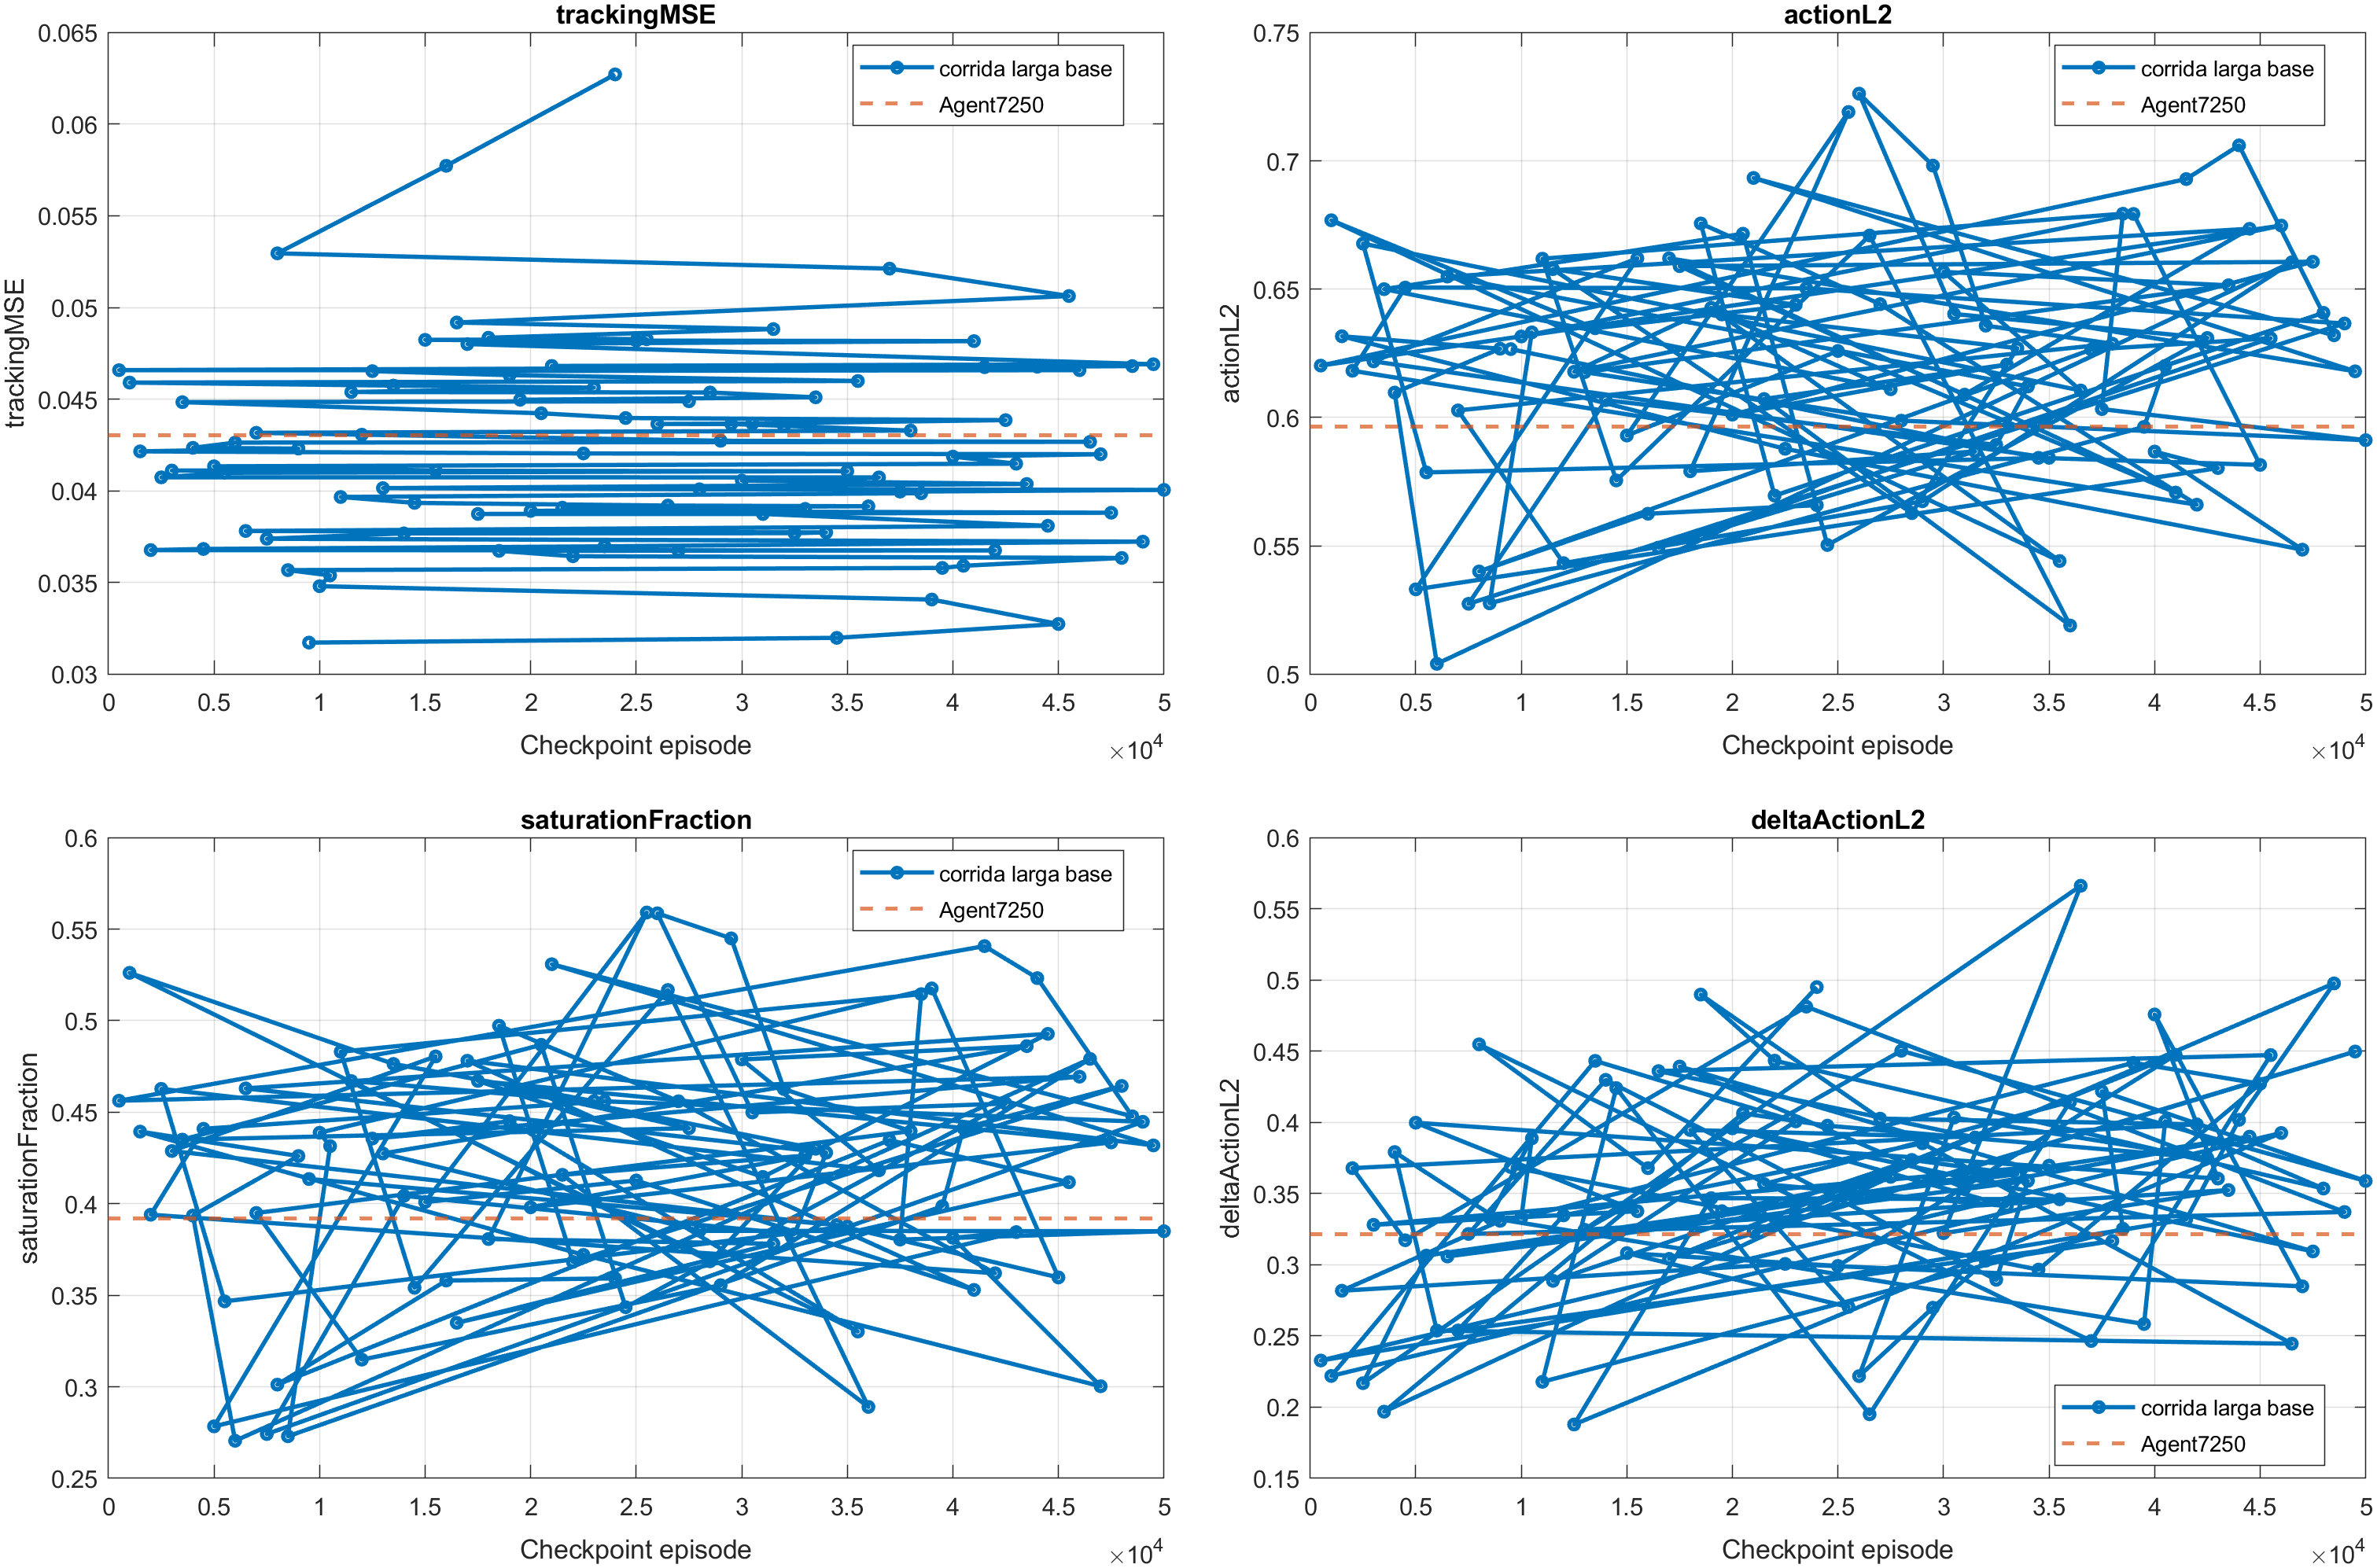
\includegraphics[width=\linewidth]{figures/agent7250_longrun_checkpoint_evolution_20260404.png}
\caption{Evoluci\'on de m\'etricas por checkpoint en la corrida larga base.}
\label{fig:base_audit}
\end{figure}

La auditor\'ia completa sobre todos los checkpoints encontr\'o como mejor candidato a \texttt{Agent39000}. En la fase completa de auditor\'ia obtuvo:
\begin{itemize}
    \item \texttt{trackingMSE = 0.041691}
    \item \texttt{trackingMAE} no usado para ranking, pero consistente con mejora local
    \item \texttt{actionL2 = 0.586194}
    \item \texttt{saturationFraction = 0.366878}
    \item \texttt{deltaActionL2 = 0.369051}
    \item estado de auditor\'ia: \texttt{ConditionA}
\end{itemize}

Es decir, \textbf{dentro} de la corrida larga base s\'i apareci\'o un checkpoint prometedor. El problema fue que esa promesa no sobrevivi\'o al retest final independiente.

\subsection*{Resultado final de la corrida base}
\begin{figure}[H]
\centering
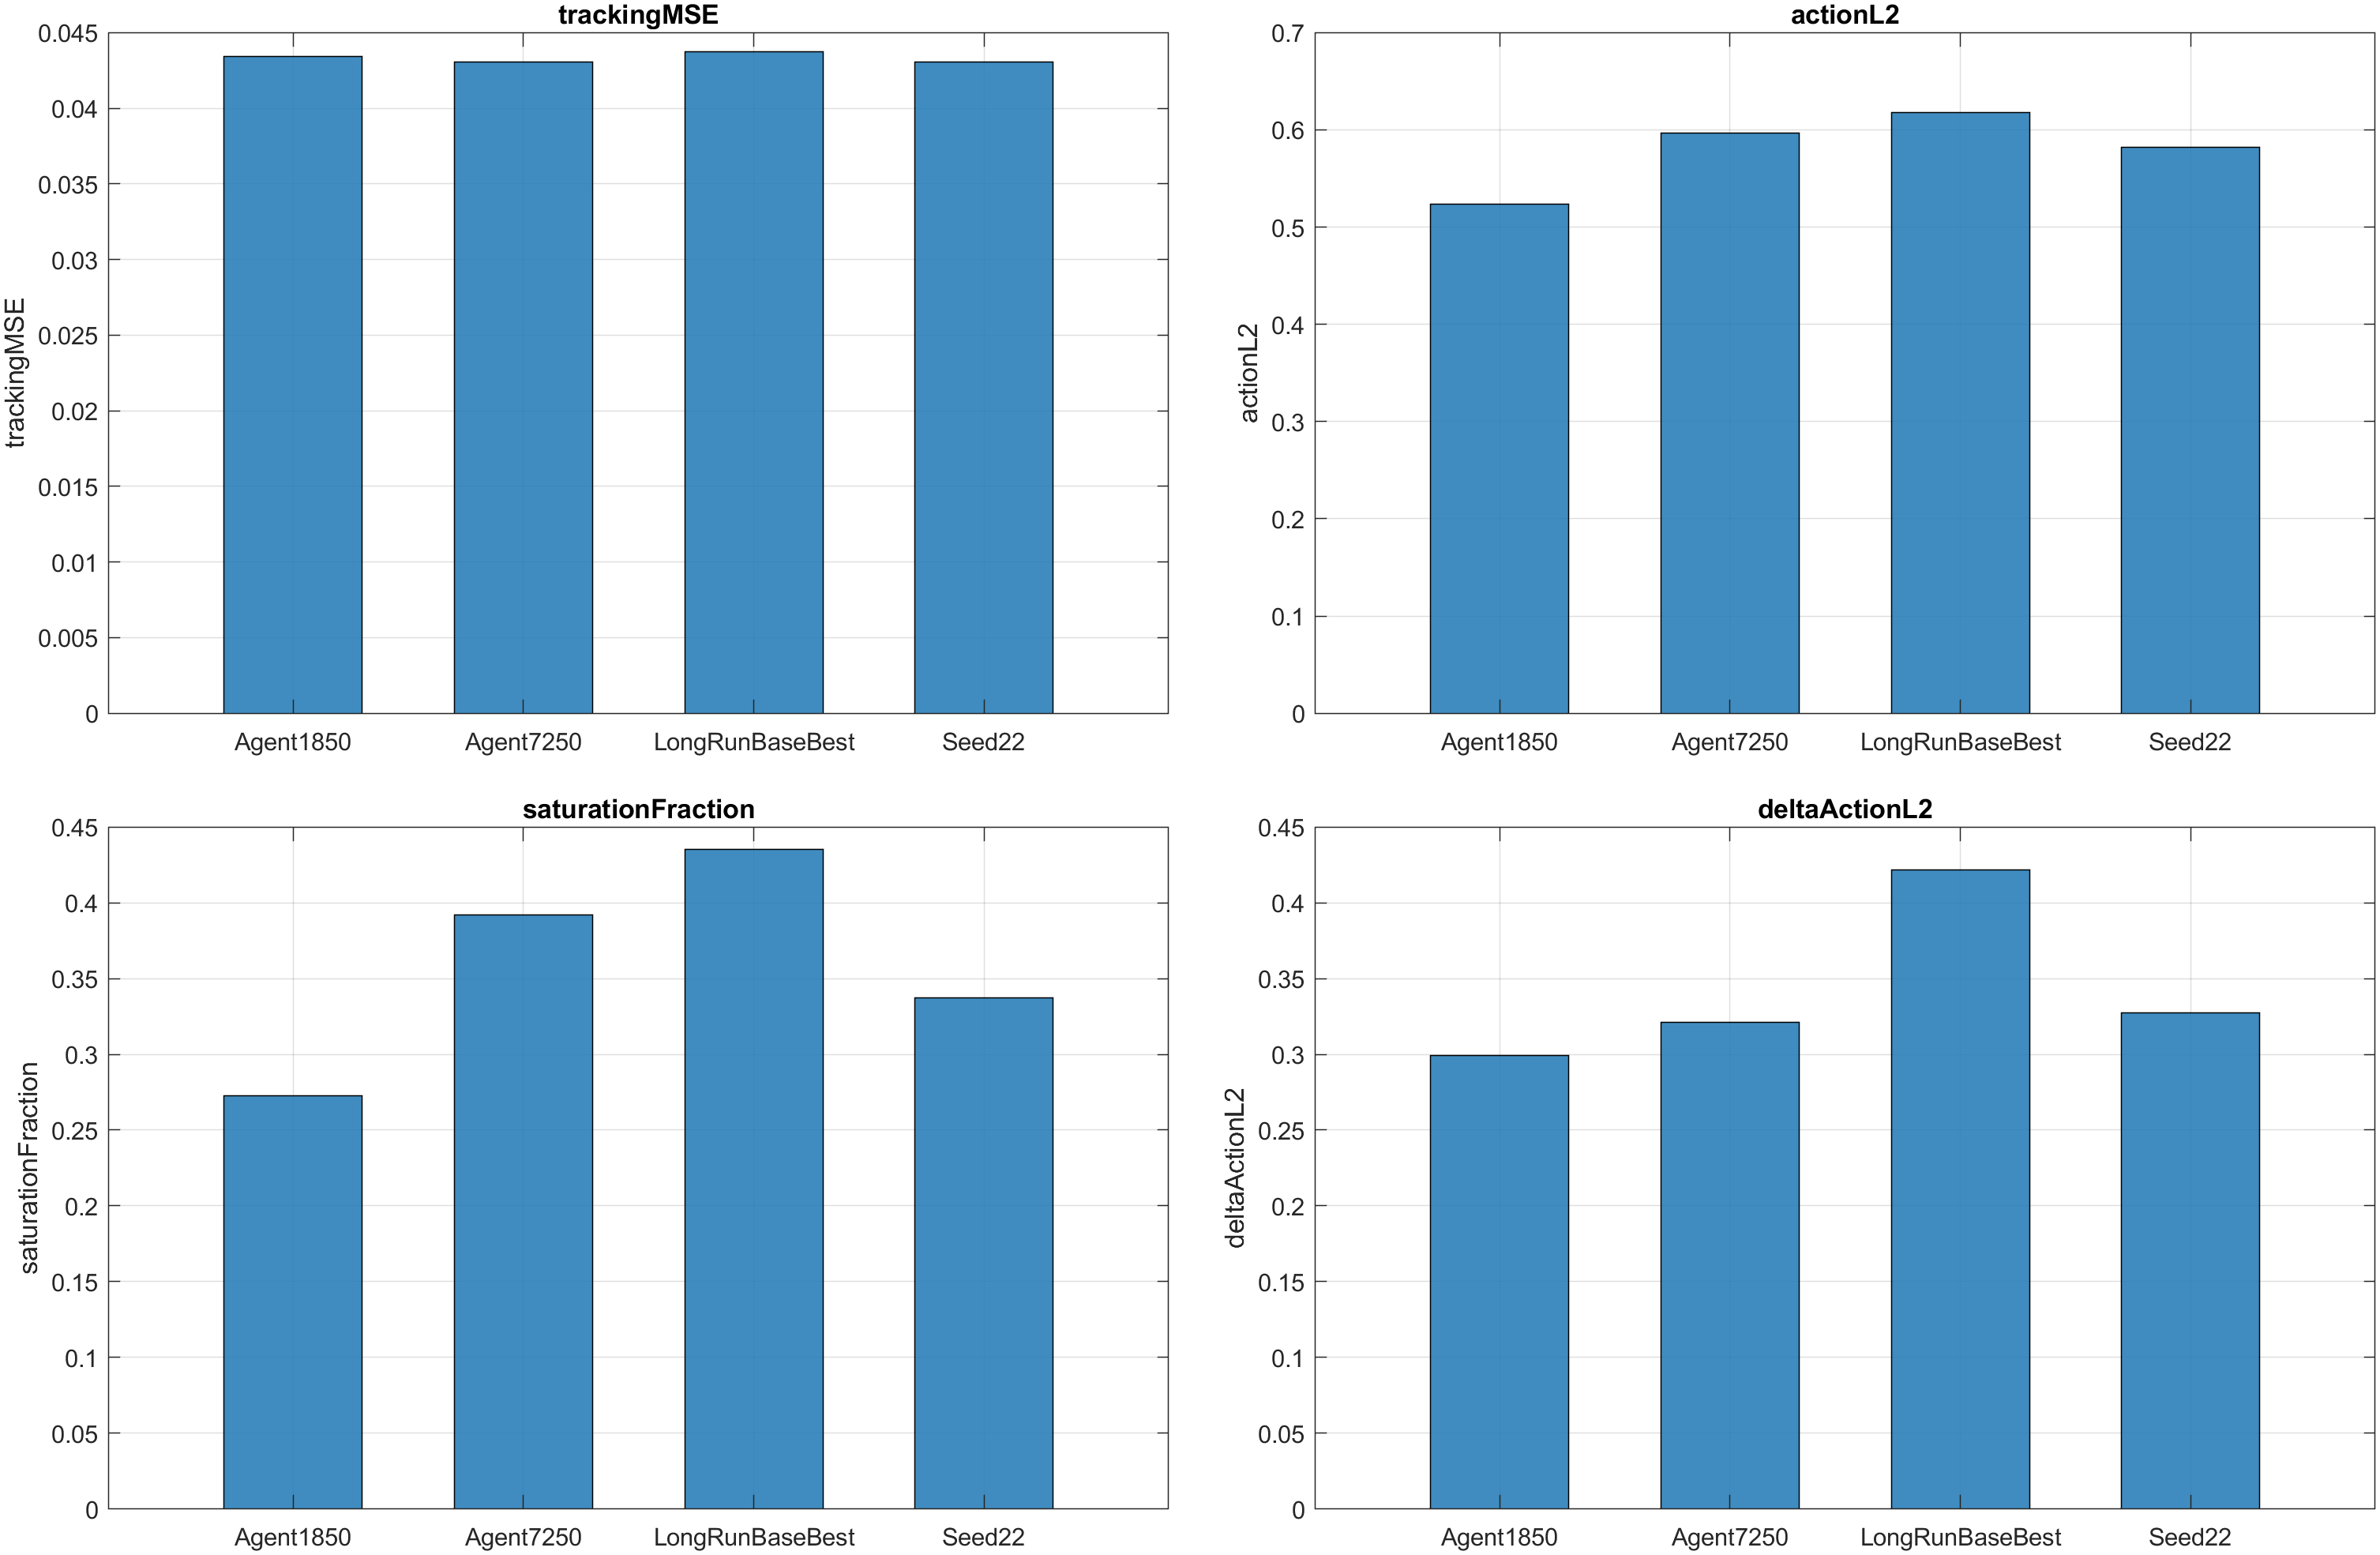
\includegraphics[width=\linewidth]{figures/agent7250_longrun_candidate_comparison_20260404.png}
\caption{Comparaci\'on final de la corrida larga base contra los candidatos relevantes del proyecto.}
\label{fig:base_comparison}
\end{figure}

\begin{table}[H]
\centering
\caption{Resultado final del mejor checkpoint de la corrida larga base}
\scriptsize
\begin{tabularx}{\linewidth}{>{\raggedright\arraybackslash}p{1.7cm} c c c c c >{\raggedright\arraybackslash}p{1.8cm}}
\toprule
Candidato & trackingMSE & trackingMAE & actionL2 & saturation & deltaActionL2 & Estado \\
\midrule
\texttt{Agent7250} & 0.043045 & 0.160336 & 0.596444 & 0.392086 & 0.321385 & Referencia \\
\texttt{Agent39000} & 0.043727 & 0.161297 & 0.618205 & 0.435191 & 0.421769 & Rejected \\
\bottomrule
\end{tabularx}
\end{table}

En el retest final de 50 simulaciones, la corrida larga base qued\'o \texttt{Rejected}. El mejor checkpoint largo:
\begin{itemize}
    \item empeor\'o el tracking frente a \texttt{Agent7250};
    \item aument\'o el esfuerzo de acci\'on;
    \item aument\'o la saturaci\'on;
    \item y empeor\'o de forma marcada la suavidad de acci\'on.
\end{itemize}

Por eso, esta corrida \textbf{no produjo una nueva base de trabajo} y no justific\'o abrir una residual sobre su mejor checkpoint.

\section*{Corrida larga residual sobre \texttt{Agent7250}}
\subsection*{Configuraci\'on}
La corrida residual larga mantuvo la receta \texttt{Residual Lift} sobre \texttt{Agent7250}, extendiendo el entrenamiento hasta 50000 episodios con la misma filosof\'ia exploratoria: ver qu\'e pasa a futuro, no solo intentar ganar.

\begin{table}[H]
\centering
\caption{Configuraci\'on principal de la corrida larga residual}
\begin{tabularx}{\linewidth}{lY}
\toprule
Elemento & Valor \\
\midrule
Carpeta experimental & \texttt{Agentes/agente\_corrida\_larga26-04-01 19 14 56} \\
Agente & \texttt{td3\_residual\_lift} \\
Checkpoint base congelado & \texttt{Agent7250} \\
Escala residual & $\alpha_{\mathrm{res}} = 0.20$ \\
Exploraci\'on & $0.02 / 0.002 / 10^{-4}$ \\
Episodios de entrenamiento & 50000 \\
Guardado de checkpoints & cada 500 episodios \\
Guardado de episodios & cada 500 episodios \\
Plots de entrenamiento & \texttt{none} \\
Semilla controlada & no (\texttt{randomSeed = NaN}) \\
\bottomrule
\end{tabularx}
\end{table}

\subsection*{Curva de entrenamiento}
\begin{figure}[H]
\centering
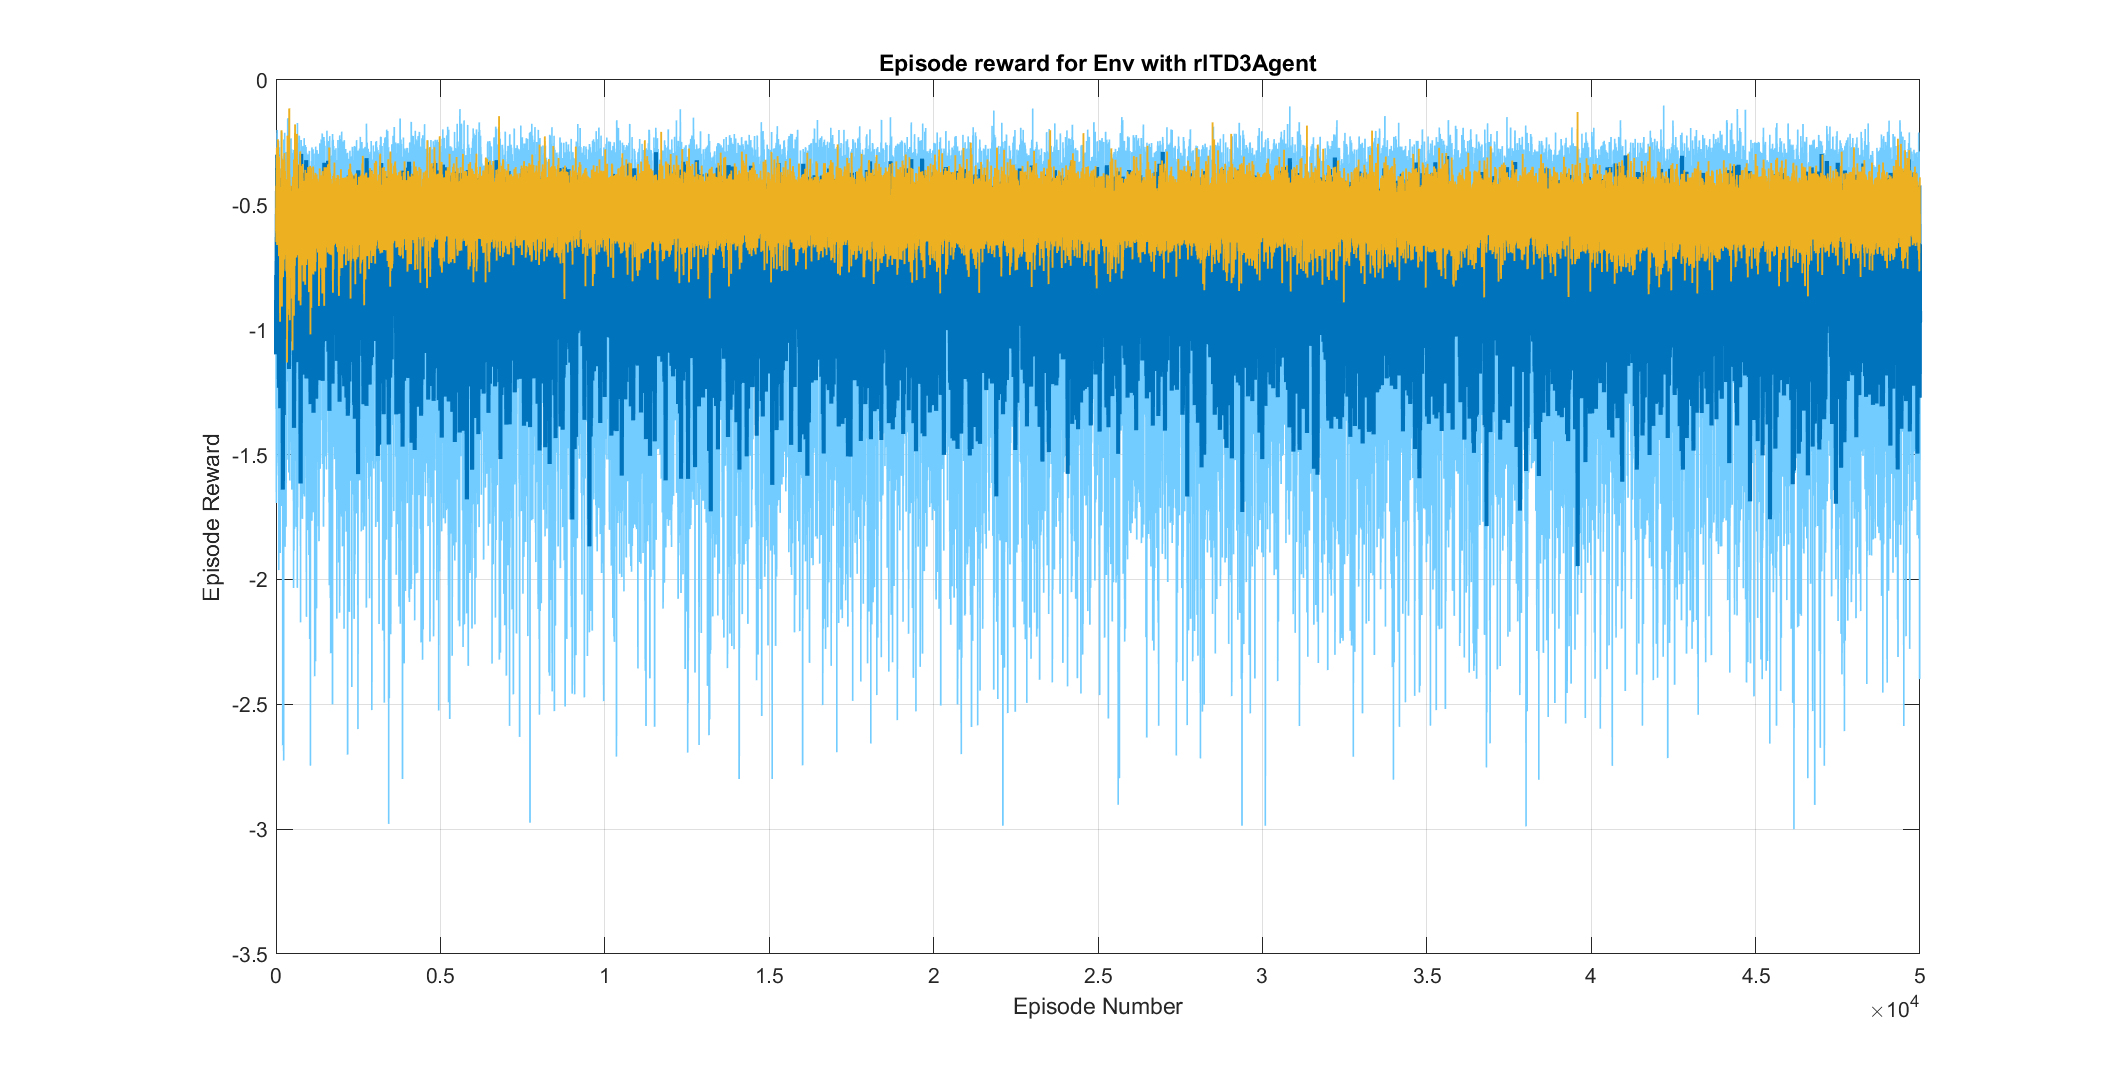
\includegraphics[width=\linewidth]{figures/longrun_residual_training_progress_20260402.png}
\caption{Curva de entrenamiento de la corrida larga residual.}
\label{fig:res_training}
\end{figure}

Los datos principales reportados por la corrida residual larga fueron:
\begin{itemize}
    \item episodios totales: 50000;
    \item mejor \texttt{AverageReward}: \(-0.287762\) en el episodio 26969;
    \item \texttt{AverageReward} final: \(-0.970405\);
    \item \texttt{TotalAgentSteps} final: 711878.
\end{itemize}

La lectura es la misma que en la corrida base: el mejor comportamiento medio apareci\'o antes del final y luego hubo deterioro. Otra vez, el resultado importante no es una mejora terminal sino la evidencia de que \textbf{una extensi\'on temporal muy larga puede entrar en meseta y luego derivar}.

\subsection*{Auditor\'ia de toda la trayectoria}
\begin{figure}[H]
\centering
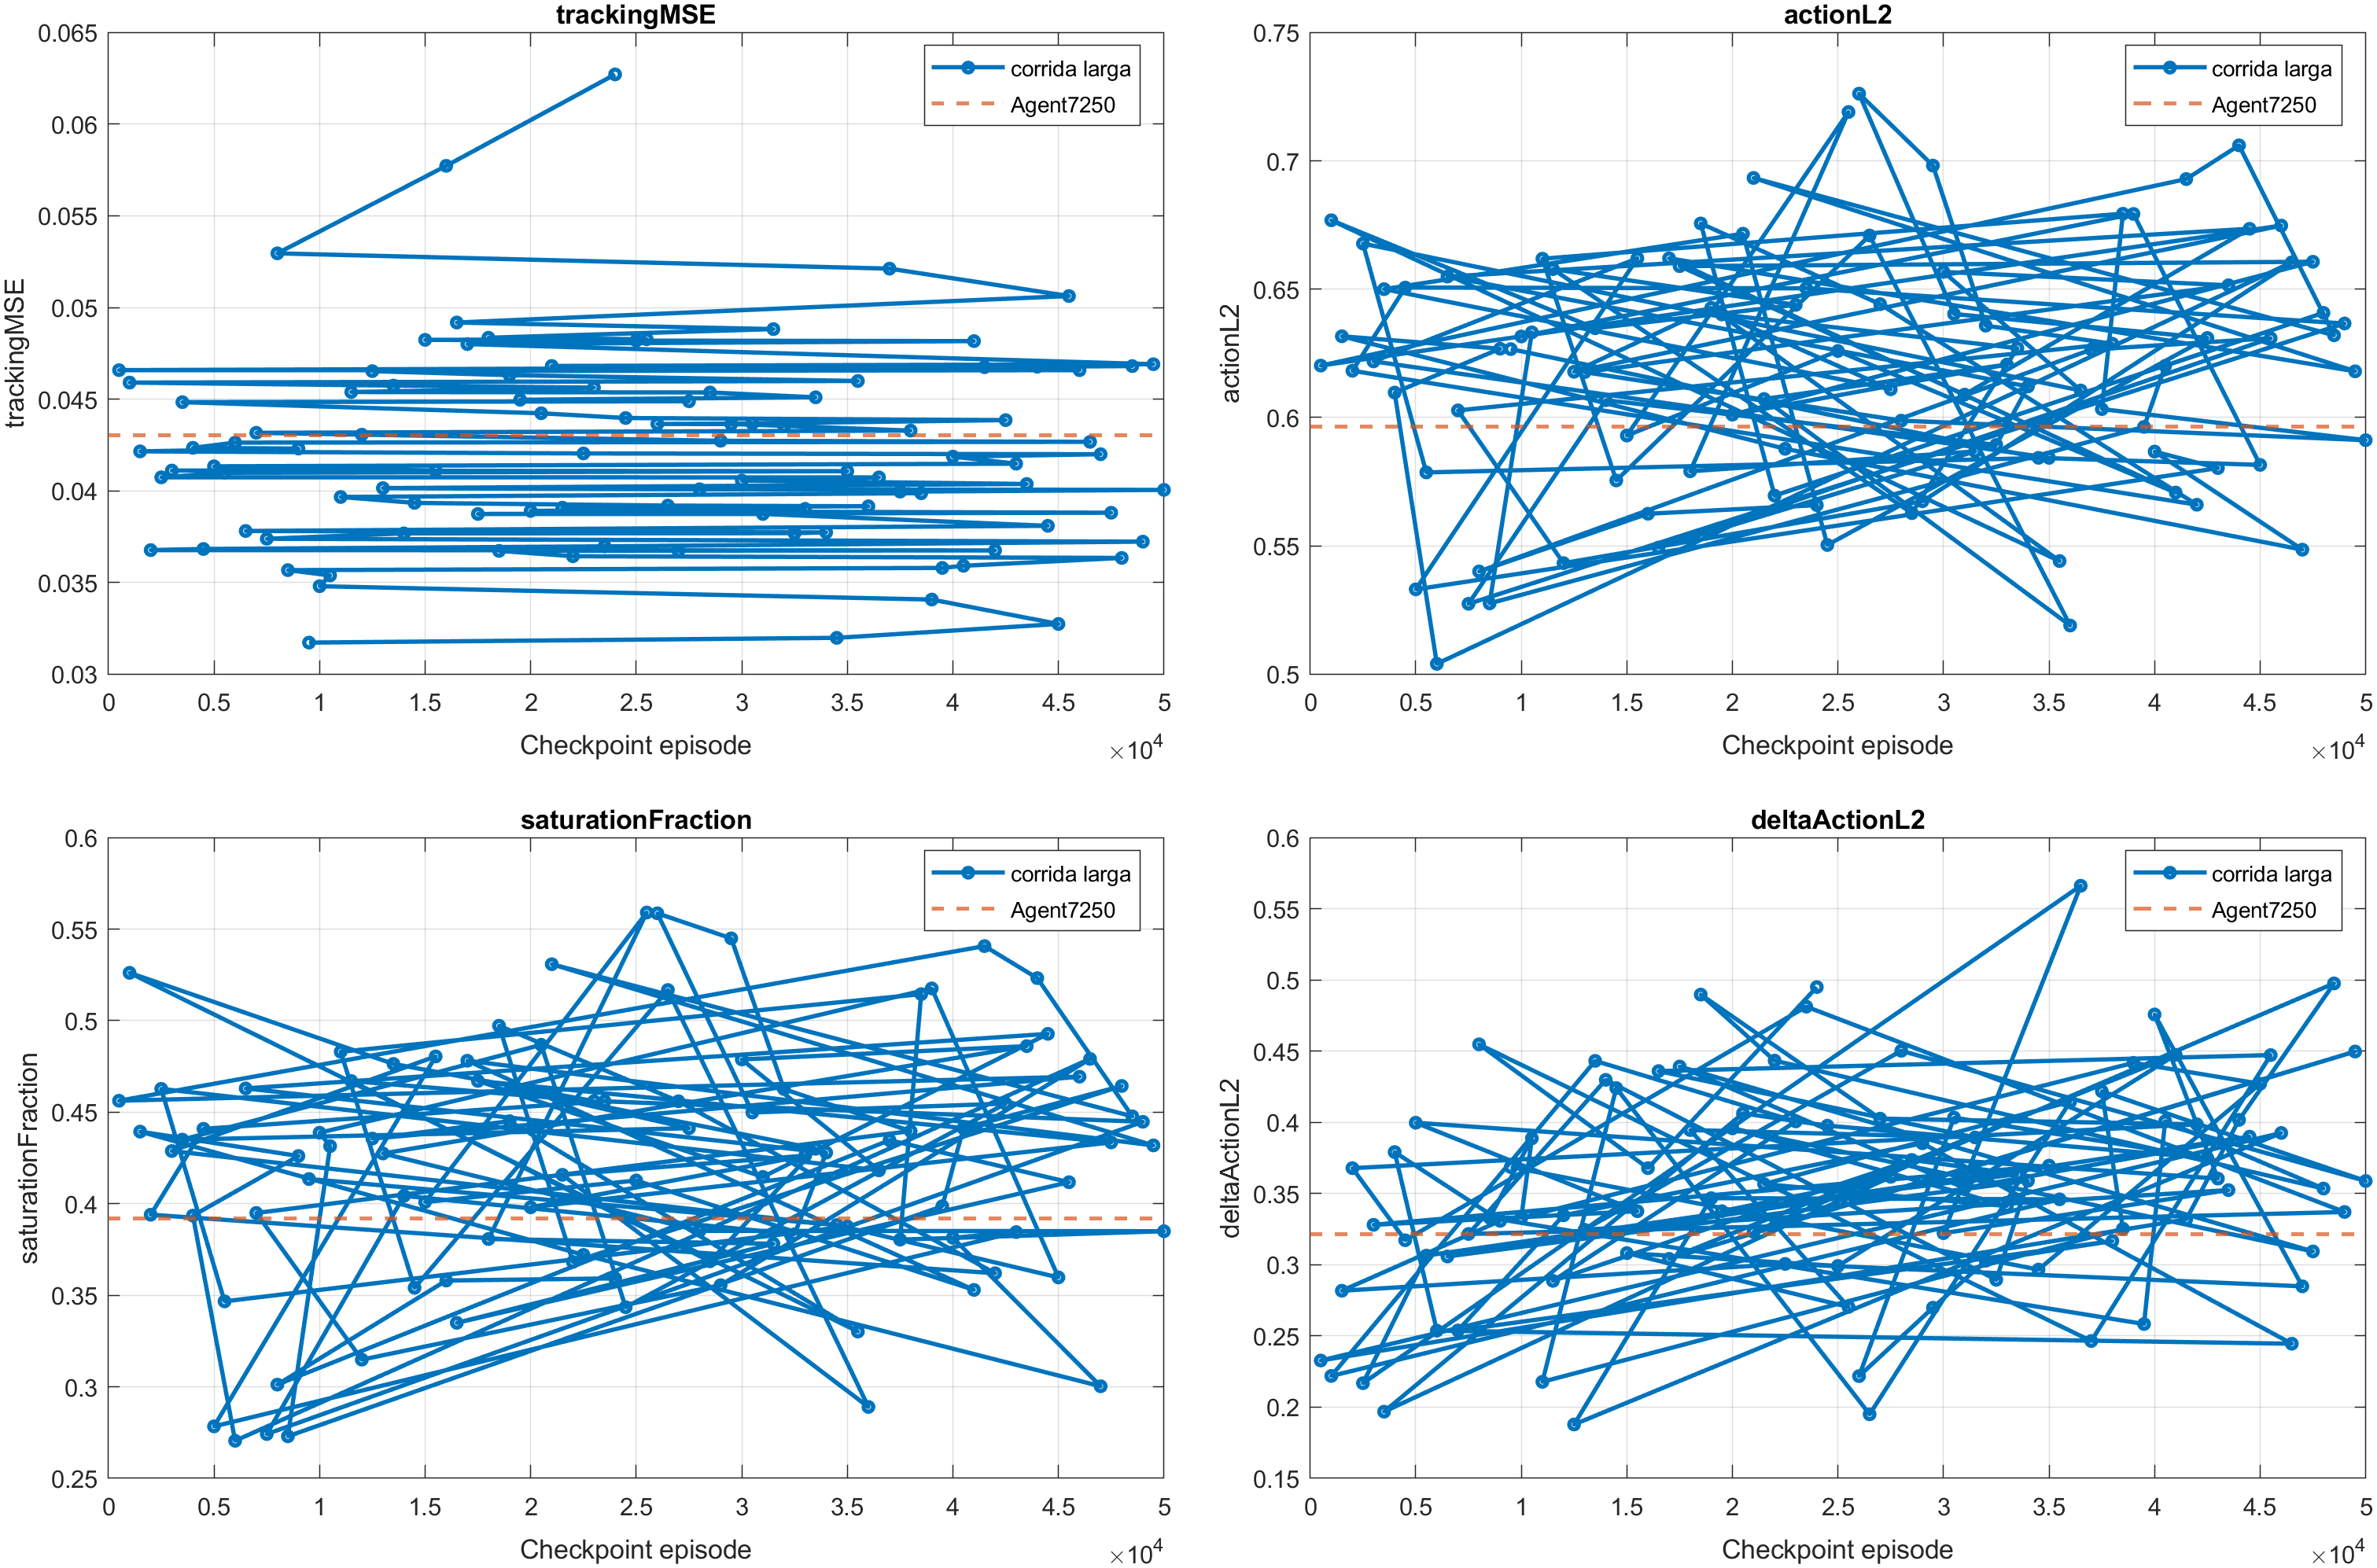
\includegraphics[width=\linewidth]{figures/longrun_residual_checkpoint_evolution_20260402.png}
\caption{Evoluci\'on de m\'etricas por checkpoint en la corrida larga residual.}
\label{fig:res_audit}
\end{figure}

La auditor\'ia completa de la corrida residual tambi\'en seleccion\'o \texttt{Agent39000} como mejor checkpoint. En fase completa obtuvo:
\begin{itemize}
    \item \texttt{trackingMSE = 0.041691}
    \item \texttt{actionL2 = 0.586194}
    \item \texttt{saturationFraction = 0.366878}
    \item \texttt{deltaActionL2 = 0.369051}
    \item estado de auditor\'ia: \texttt{ConditionA}
\end{itemize}

Esto mostr\'o que, incluso en el residual, la mejor zona auditada apareci\'o cerca del episodio 39000 y no al final de la corrida.

\subsection*{Resultado final de la corrida residual}
\begin{figure}[H]
\centering
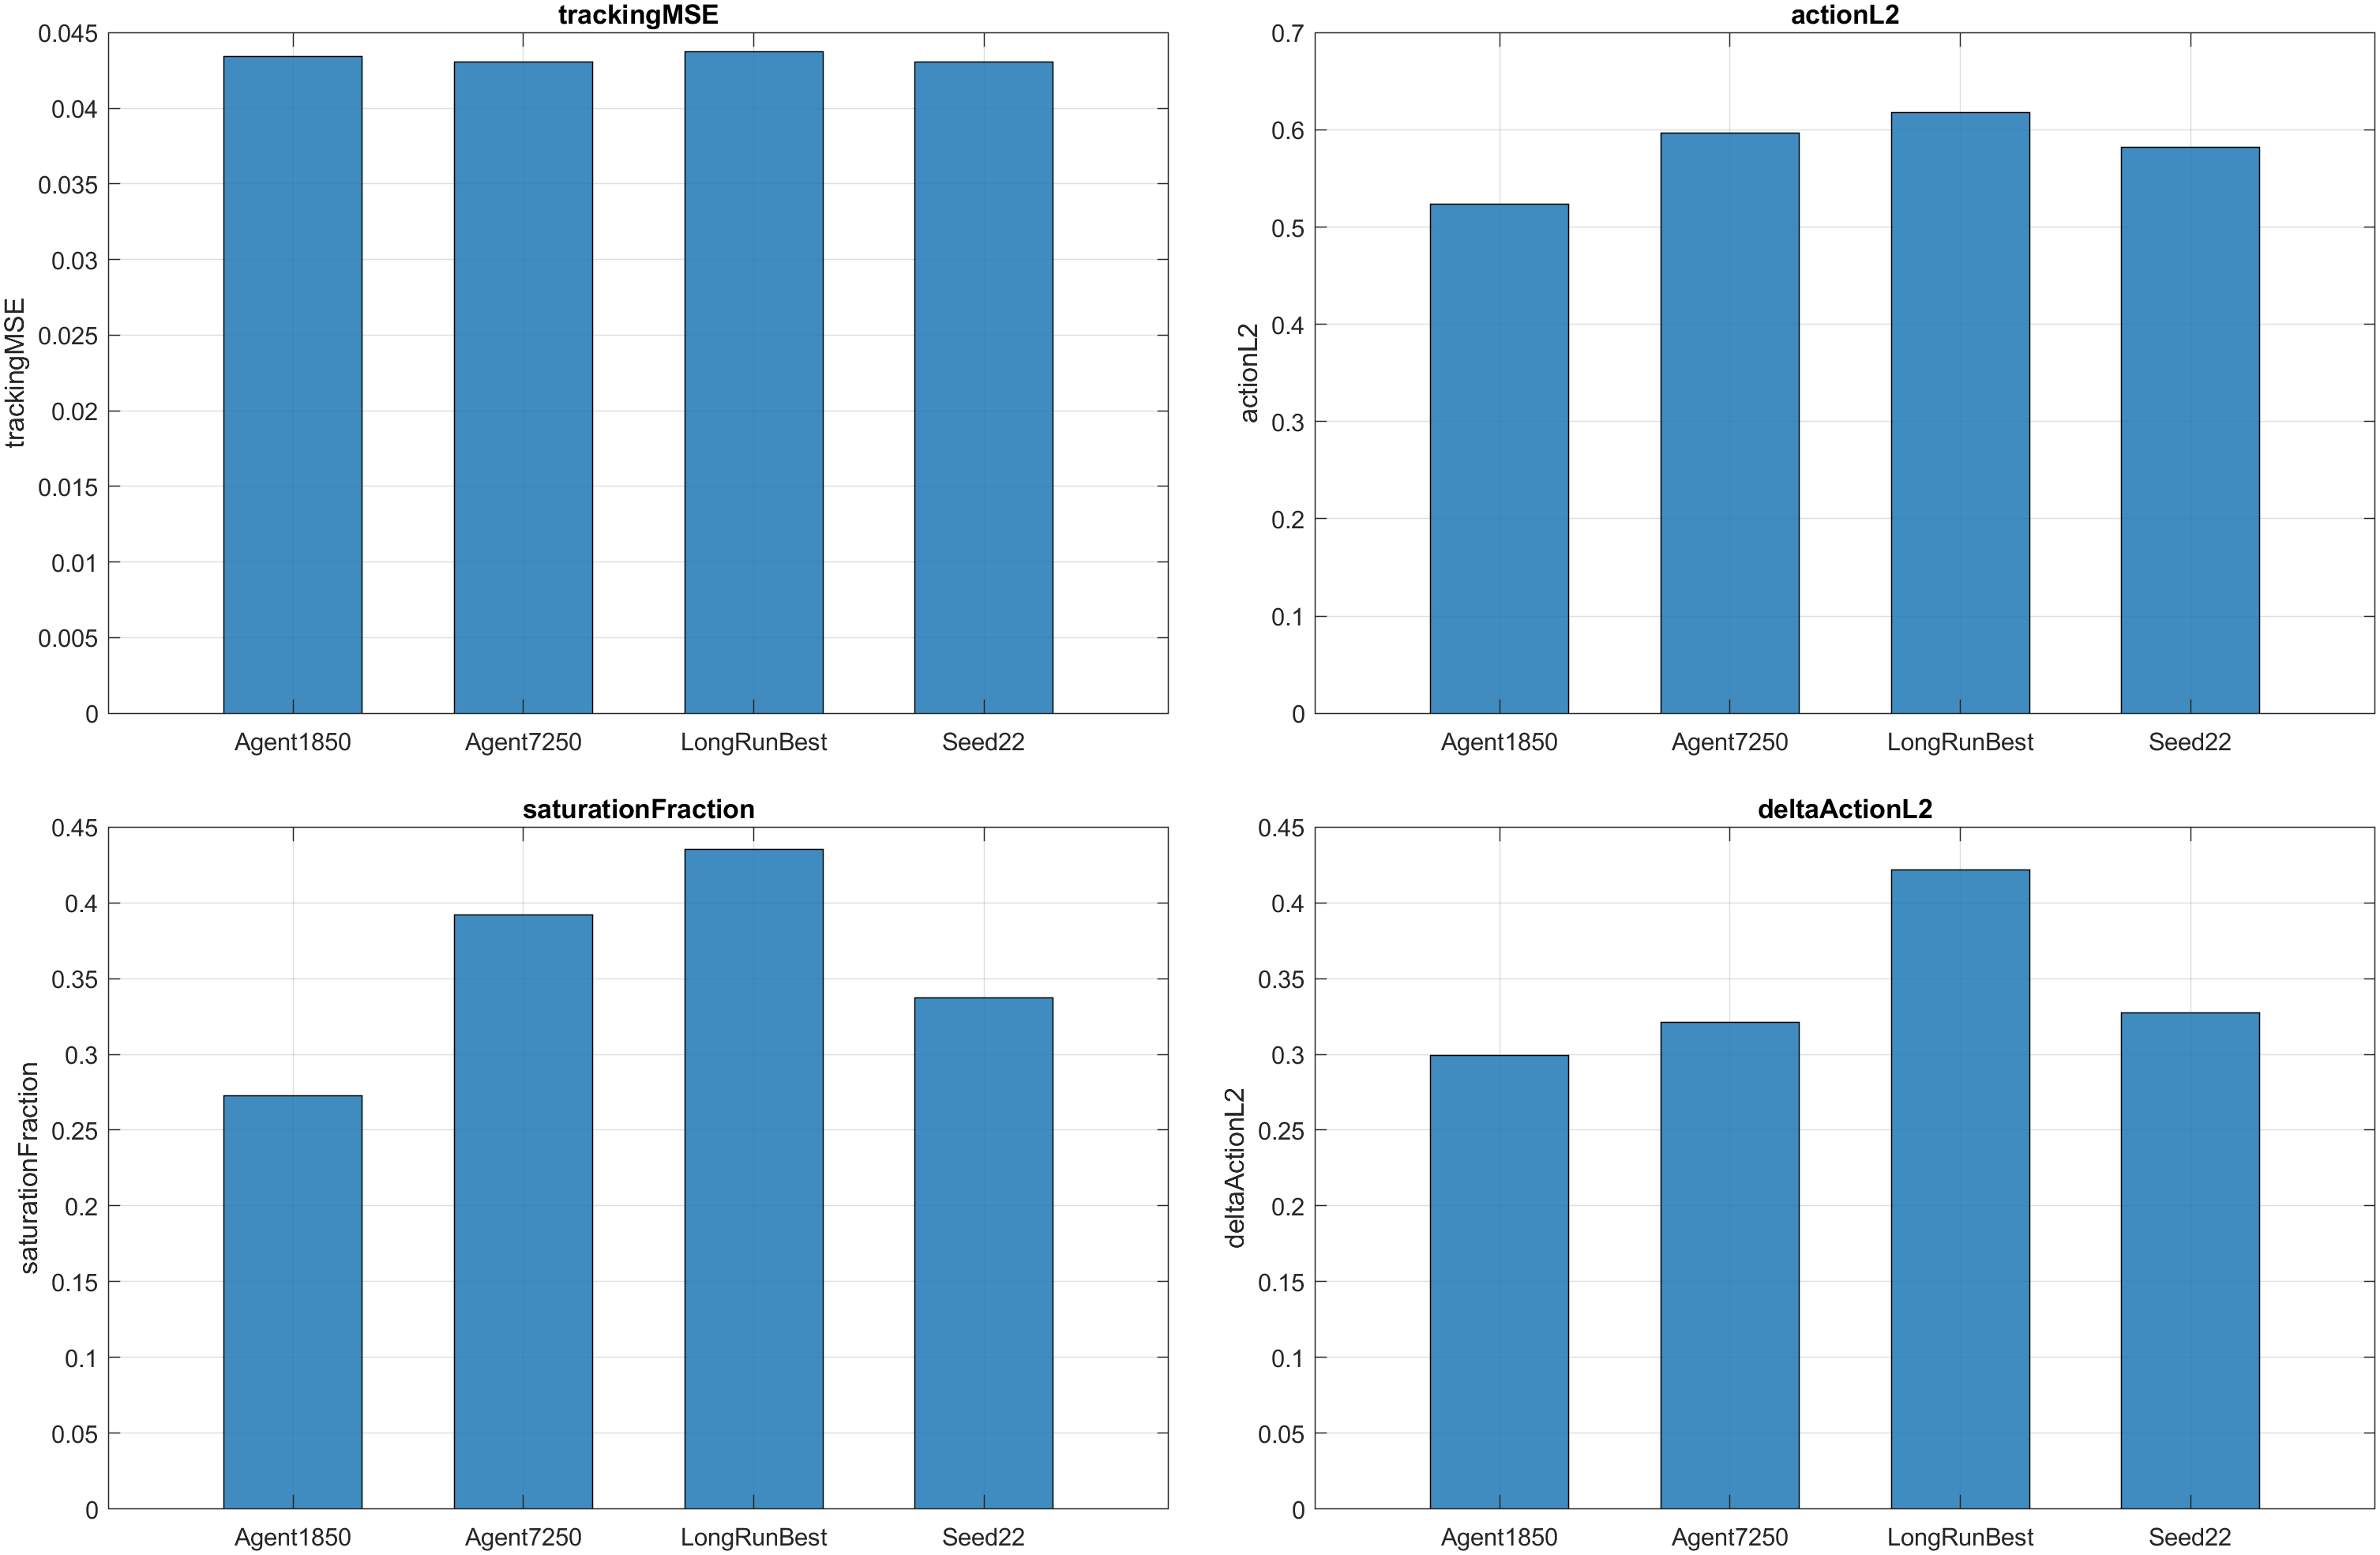
\includegraphics[width=\linewidth]{figures/longrun_residual_candidate_comparison_20260402.png}
\caption{Comparaci\'on final de la corrida larga residual contra los candidatos relevantes del proyecto.}
\label{fig:res_comparison}
\end{figure}

\begin{table}[H]
\centering
\caption{Resultado final del mejor checkpoint de la corrida larga residual}
\scriptsize
\begin{tabularx}{\linewidth}{>{\raggedright\arraybackslash}p{1.7cm} c c c c c >{\raggedright\arraybackslash}p{1.8cm}}
\toprule
Candidato & trackingMSE & trackingMAE & actionL2 & saturation & deltaActionL2 & Estado \\
\midrule
\texttt{Agent7250} & 0.043045 & 0.160336 & 0.596444 & 0.392086 & 0.321385 & Referencia \\
\texttt{Agent39000} & 0.043727 & 0.161297 & 0.618205 & 0.435191 & 0.421769 & Rejected \\
\bottomrule
\end{tabularx}
\end{table}

En el retest final independiente, la corrida residual larga tambi\'en termin\'o \texttt{Rejected}. Esto significa que la extensi\'on hasta 50000 episodios \textbf{no consolid\'o} un residual mejor que los candidatos ya conocidos.

\section*{S\'intesis conjunta de las dos corridas largas}
La Tabla~\ref{tab:joint} resume las dos corridas largas bajo la misma l\'ogica de lectura.

\begin{table}[H]
\centering
\caption{Resumen conjunto de las dos corridas largas de 50000 episodios}
\label{tab:joint}
\scriptsize
\begin{tabularx}{\linewidth}{>{\raggedright\arraybackslash}p{2.35cm} c c c >{\raggedright\arraybackslash}p{1.65cm} >{\raggedright\arraybackslash}p{1.65cm} >{\raggedright\arraybackslash}p{1.35cm}}
\toprule
Corrida & Mejor AvgReward & Episodio & AvgReward final & Mejor ckpt & Estado auditor\'ia & Estado final \\
\midrule
Base sobre \texttt{Agent7250} & -0.287762 & 26969 & -0.970405 & \texttt{Agent39000} & ConditionA & Rejected \\
Residual sobre \texttt{Agent7250} & -0.287762 & 26969 & -0.970405 & \texttt{Agent39000} & ConditionA & Rejected \\
\bottomrule
\end{tabularx}
\end{table}

Operativamente, ambas corridas largas muestran el mismo patr\'on:
\begin{enumerate}
    \item el mejor comportamiento promedio aparece en una zona intermedia, no al final;
    \item la auditor\'ia puede detectar checkpoints prometedores dentro de la trayectoria;
    \item al revalidar con el protocolo final de 50 simulaciones, ese mejor checkpoint no se sostiene como nuevo l\'ider.
\end{enumerate}

Esto refuerza una lectura importante del proyecto: \textbf{seguir entrenando por mucho m\'as tiempo no garantiza una mejor pol\'itica final}. De hecho, en estas dos extensiones largas aparece evidencia compatible con meseta seguida de desaprendizaje o deriva tard\'ia.

\section*{Comparaci\'on contra los candidatos que realmente quedan vigentes}
Para fijar d\'onde conviene quedarnos, la comparaci\'on relevante no es solo entre las dos corridas largas, sino entre esas corridas y los candidatos que todav\'ia siguen vivos dentro del proyecto.

\begin{table}[H]
\centering
\caption{Candidatos vigentes del proyecto despu\'es de las dos corridas largas}
\label{tab:project_state}
\scriptsize
\begin{tabularx}{\linewidth}{>{\raggedright\arraybackslash}p{2.25cm} c c c c c >{\raggedright\arraybackslash}p{2.55cm}}
\toprule
Candidato & trackingMSE & trackingMAE & actionL2 & saturation & deltaActionL2 & Lectura \\
\midrule
\texttt{Agent7250} & 0.043045 & 0.160336 & 0.596444 & 0.392086 & 0.321385 & Benchmark oficial estable \\
\texttt{seed 22} & 0.043045 & 0.160786 & 0.582152 & 0.337475 & 0.327141 & Mejor residual reproducible (\texttt{ConditionA}) \\
\texttt{Agent1850} & 0.043445 & 0.163542 & 0.523597 & 0.272637 & 0.299262 & Mejor residual single-run hist\'orico (\texttt{ConditionB}) \\
Mejor corrida larga base & 0.043727 & 0.161297 & 0.618205 & 0.435191 & 0.421769 & Exploraci\'on temporal, no promover \\
Mejor corrida larga residual & 0.043727 & 0.161297 & 0.618205 & 0.435191 & 0.421769 & Exploraci\'on temporal, no promover \\
\bottomrule
\end{tabularx}
\end{table}

La foto final es n\'itida:
\begin{itemize}
    \item \texttt{Agent7250} sigue siendo la referencia estable del proyecto.
    \item \texttt{seed 22} sigue siendo la mejor evidencia residual reproducible.
    \item \texttt{Agent1850} sigue siendo el mejor residual single-run hist\'orico si la prioridad es el compromiso tracking-esfuerzo-saturaci\'on.
    \item Ninguna de las dos corridas largas de 50000 episodios debe promoverse como nueva base, nuevo benchmark ni nuevo residual l\'ider.
\end{itemize}

\section*{Apoyo visual de las dos corridas largas}
Las figuras siguientes no cambian el veredicto por s\'i solas, pero ayudan a cerrar la lectura cualitativa de ambas extensiones temporales. En ambos casos, la interpretaci\'on visual se mantiene subordinada a las m\'etricas finales y al retest de 50 simulaciones.

\begin{figure}[H]
\centering
\begin{minipage}[t]{0.49\linewidth}
\centering
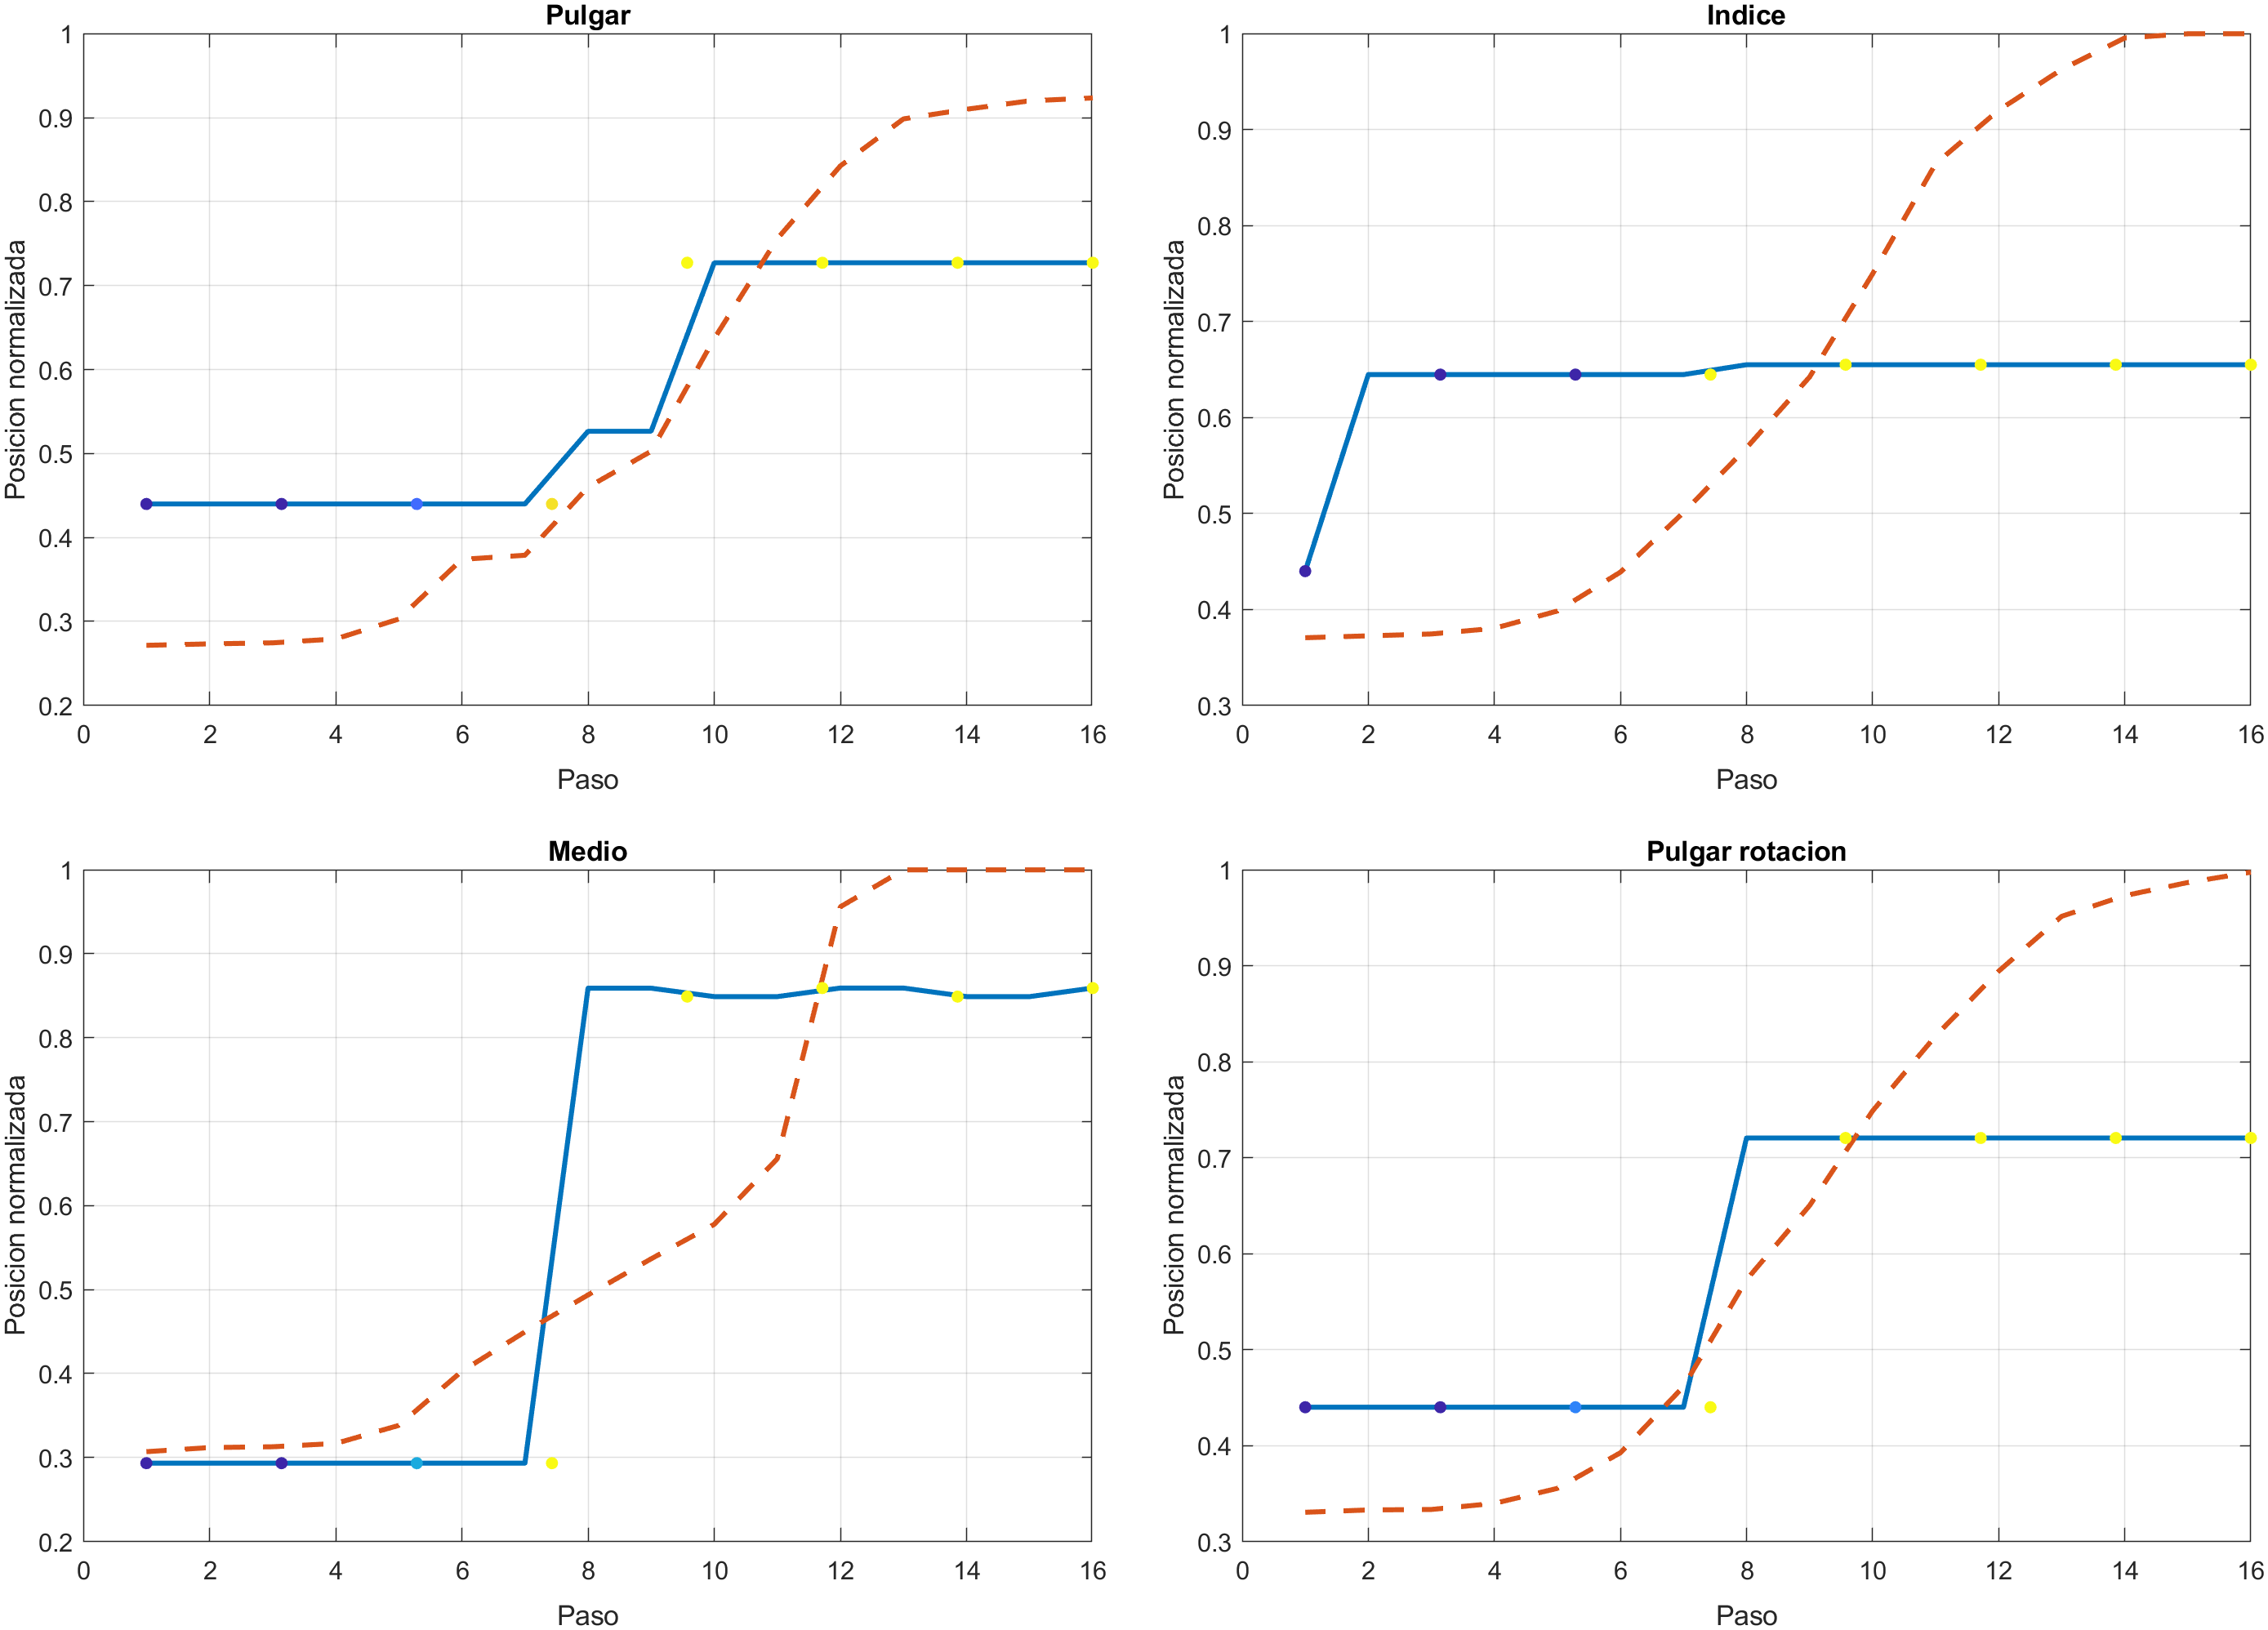
\includegraphics[width=\linewidth]{figures/agent7250_longrun_best_visual_20260404.png}
\caption*{(a) Mejor checkpoint largo base}
\end{minipage}\hfill
\begin{minipage}[t]{0.49\linewidth}
\centering
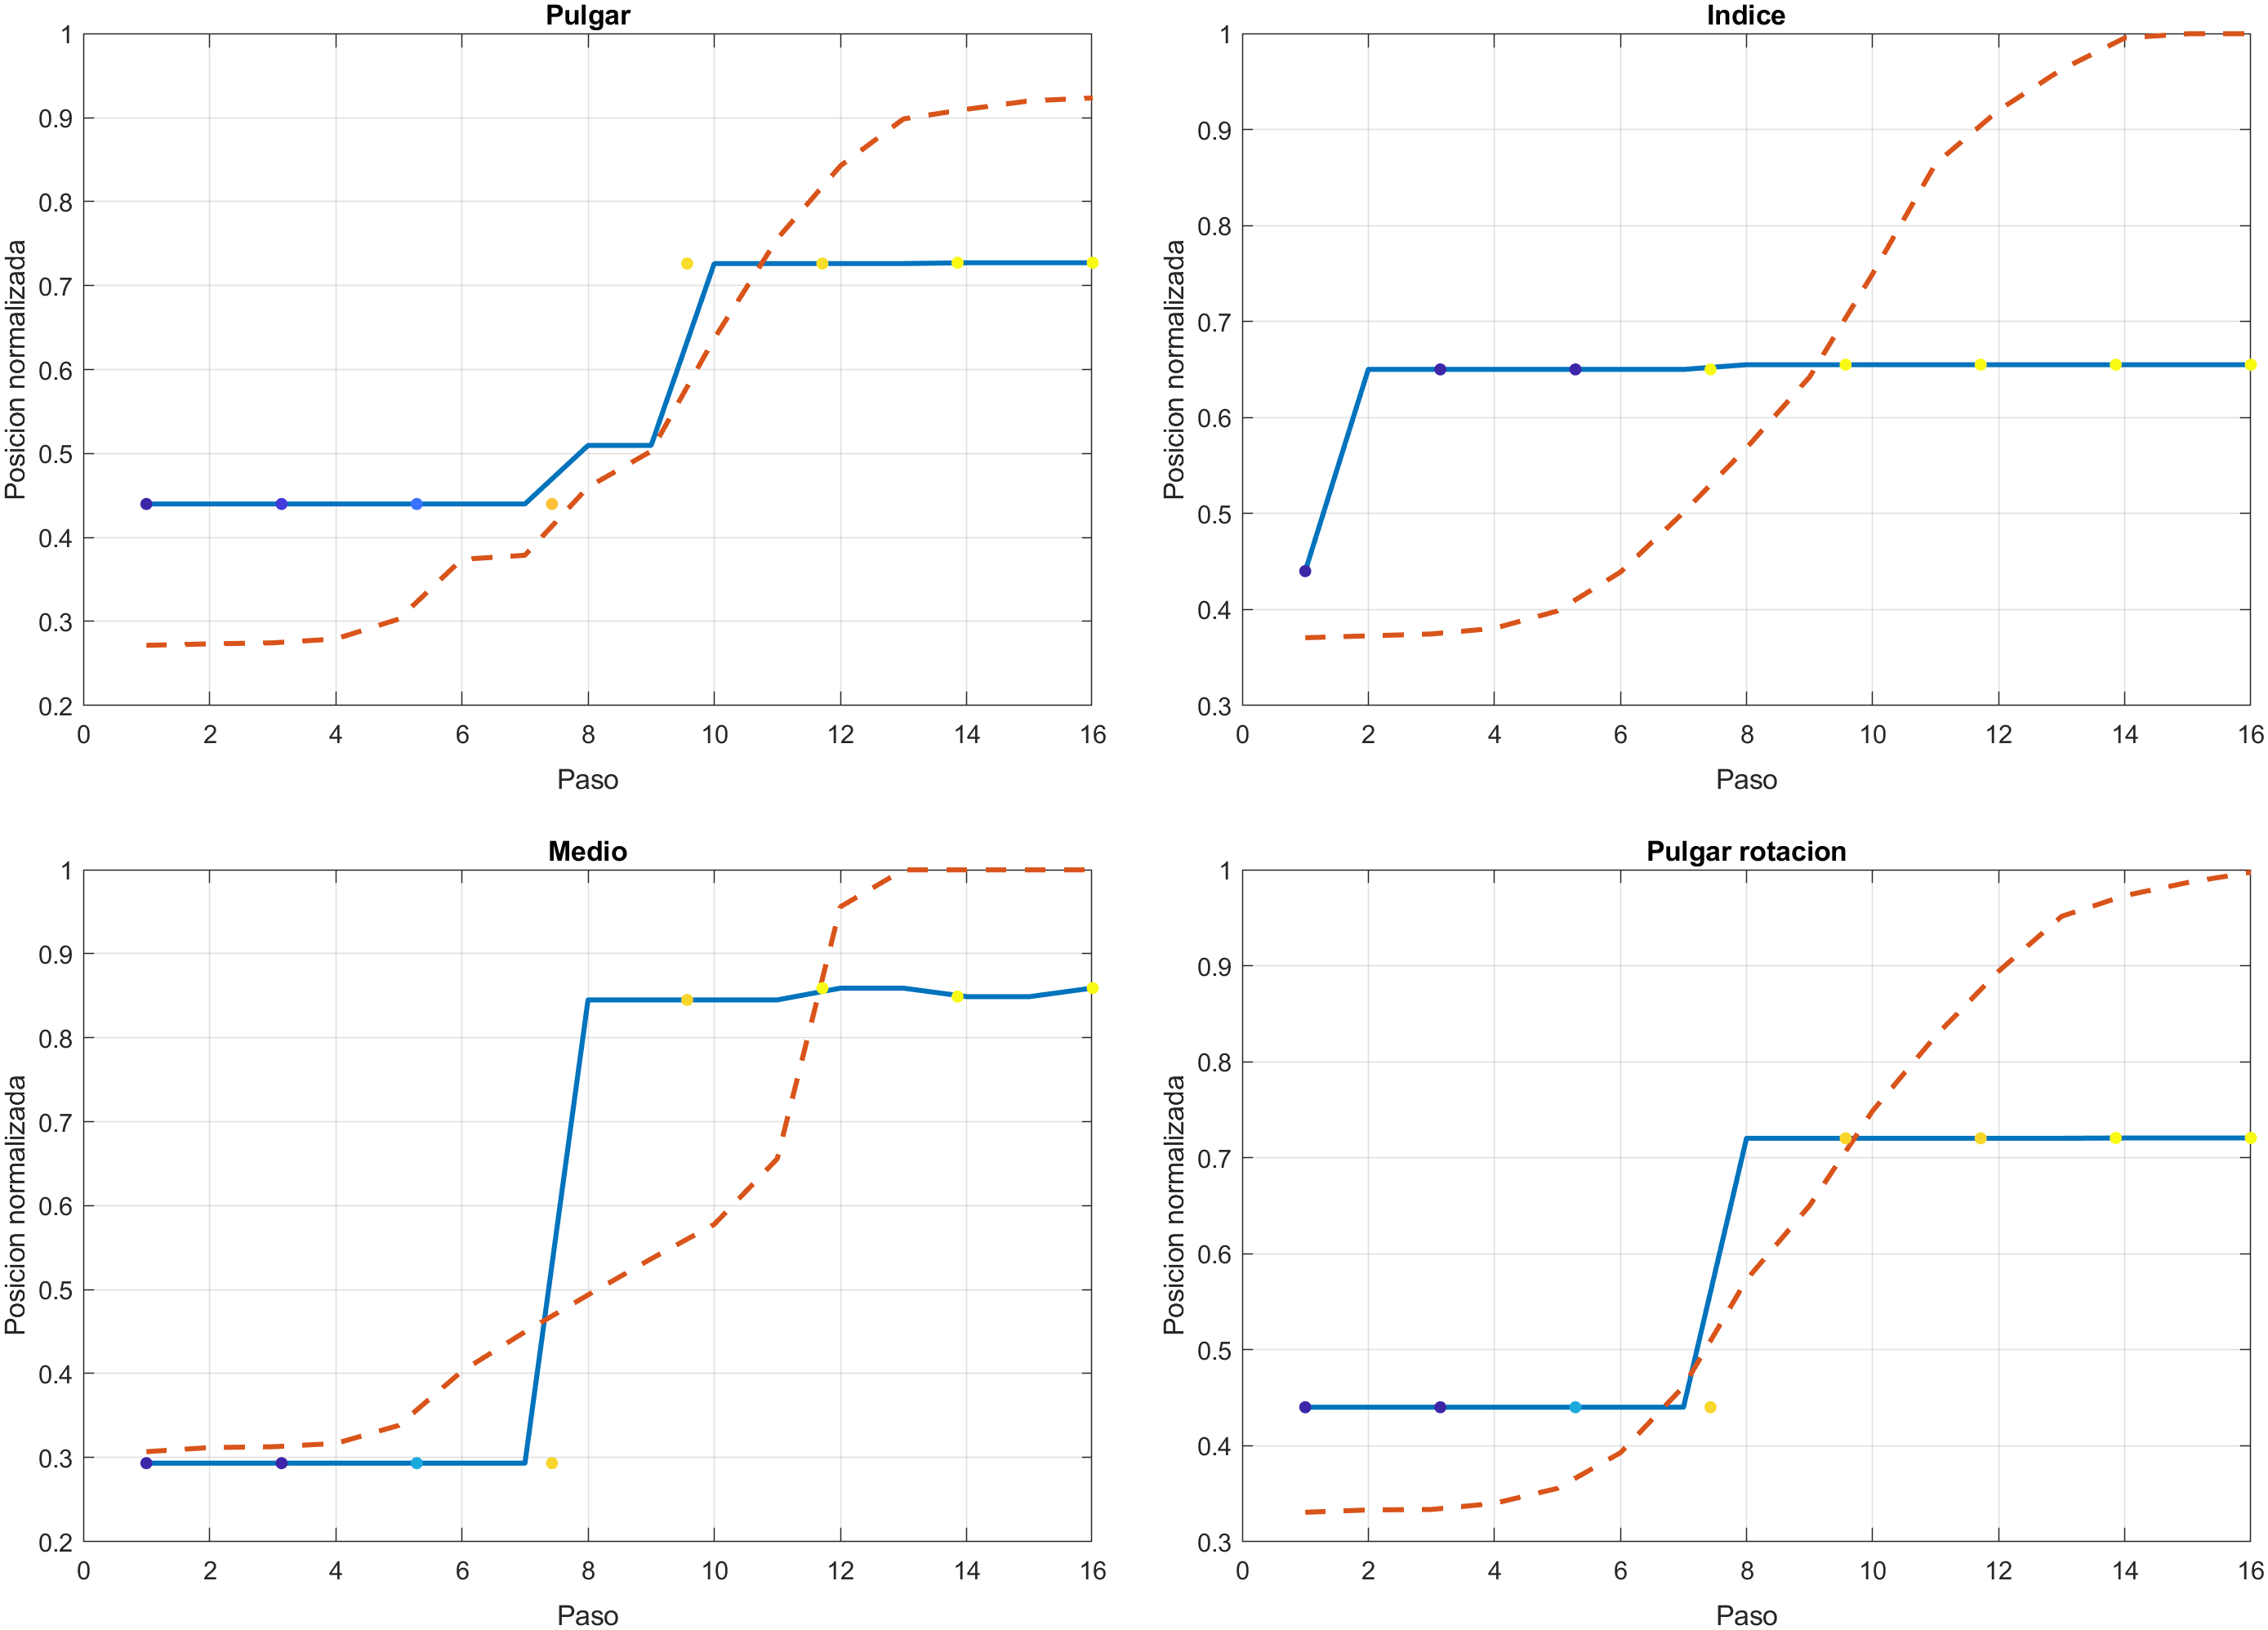
\includegraphics[width=\linewidth]{figures/agent7250_longrun_benchmark_visual_20260404.png}
\caption*{(b) Benchmark \texttt{Agent7250}}
\end{minipage}
\caption{Comparaci\'on visual cualitativa entre el mejor checkpoint de la corrida larga base y el benchmark oficial.}
\label{fig:base_visuals}
\end{figure}

\begin{figure}[H]
\centering
\begin{minipage}[t]{0.49\linewidth}
\centering
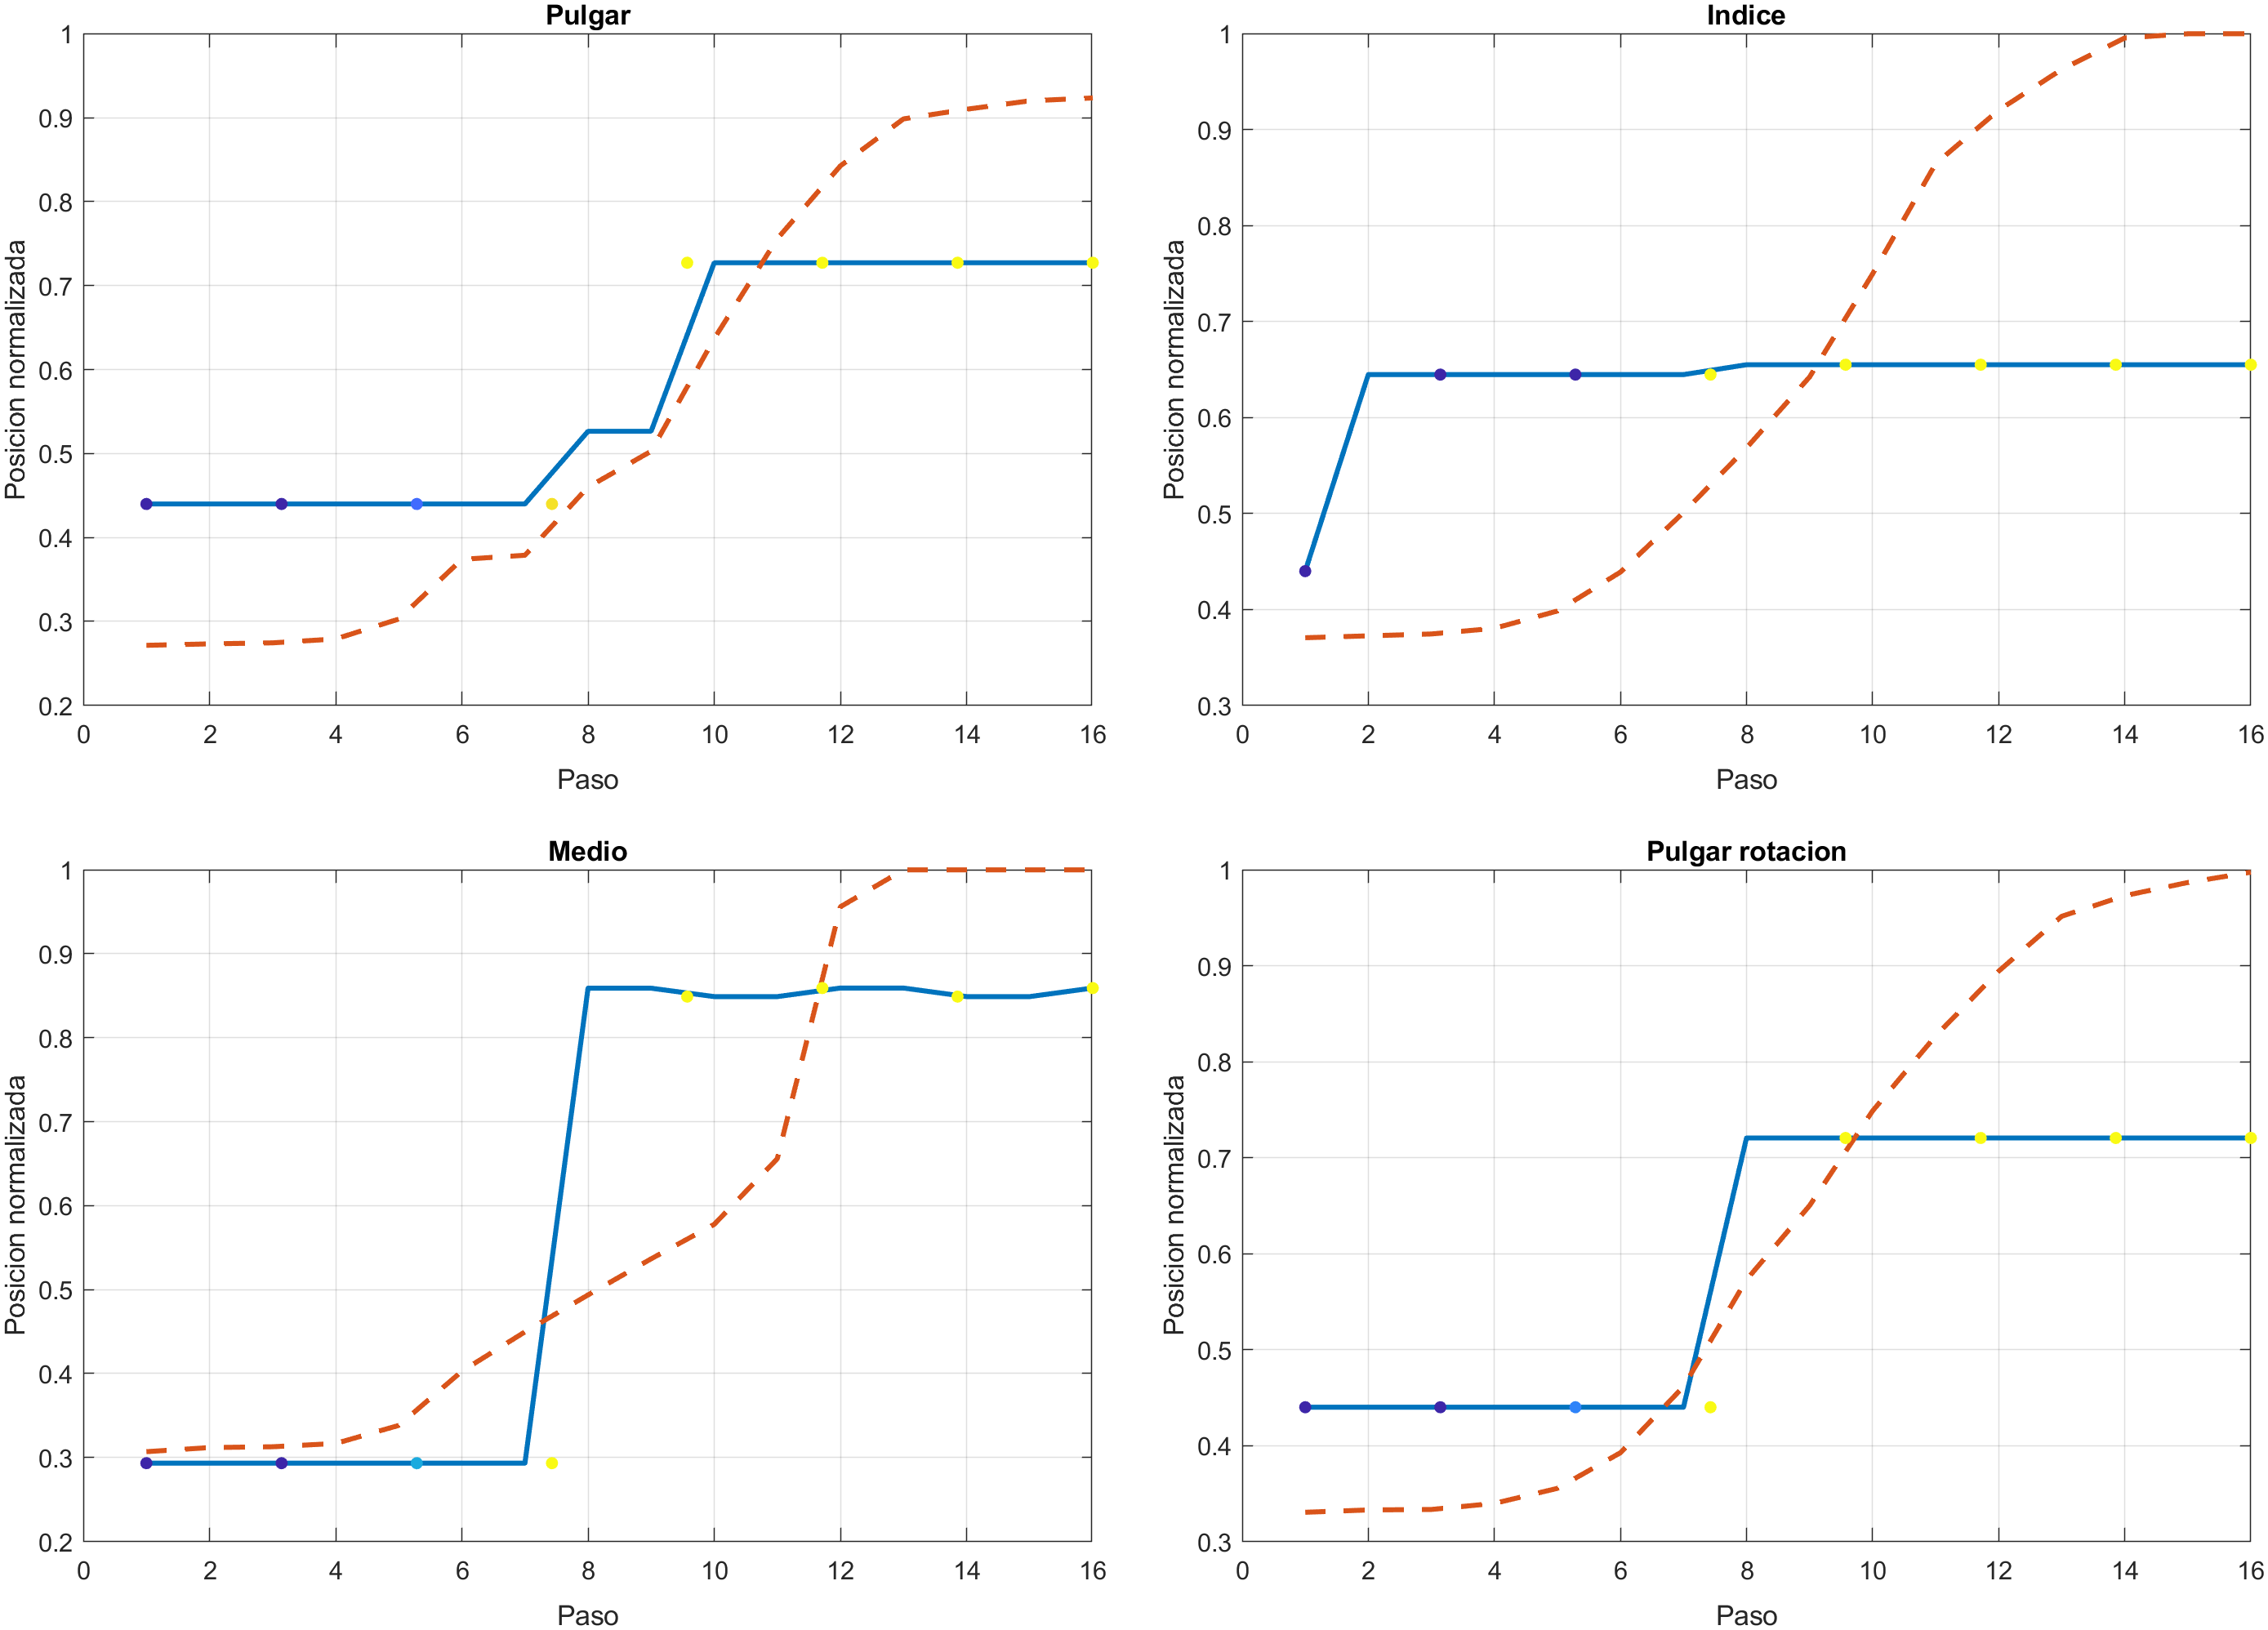
\includegraphics[width=\linewidth]{figures/longrun_residual_best_visual_20260402.png}
\caption*{(a) Mejor checkpoint largo residual}
\end{minipage}\hfill
\begin{minipage}[t]{0.49\linewidth}
\centering
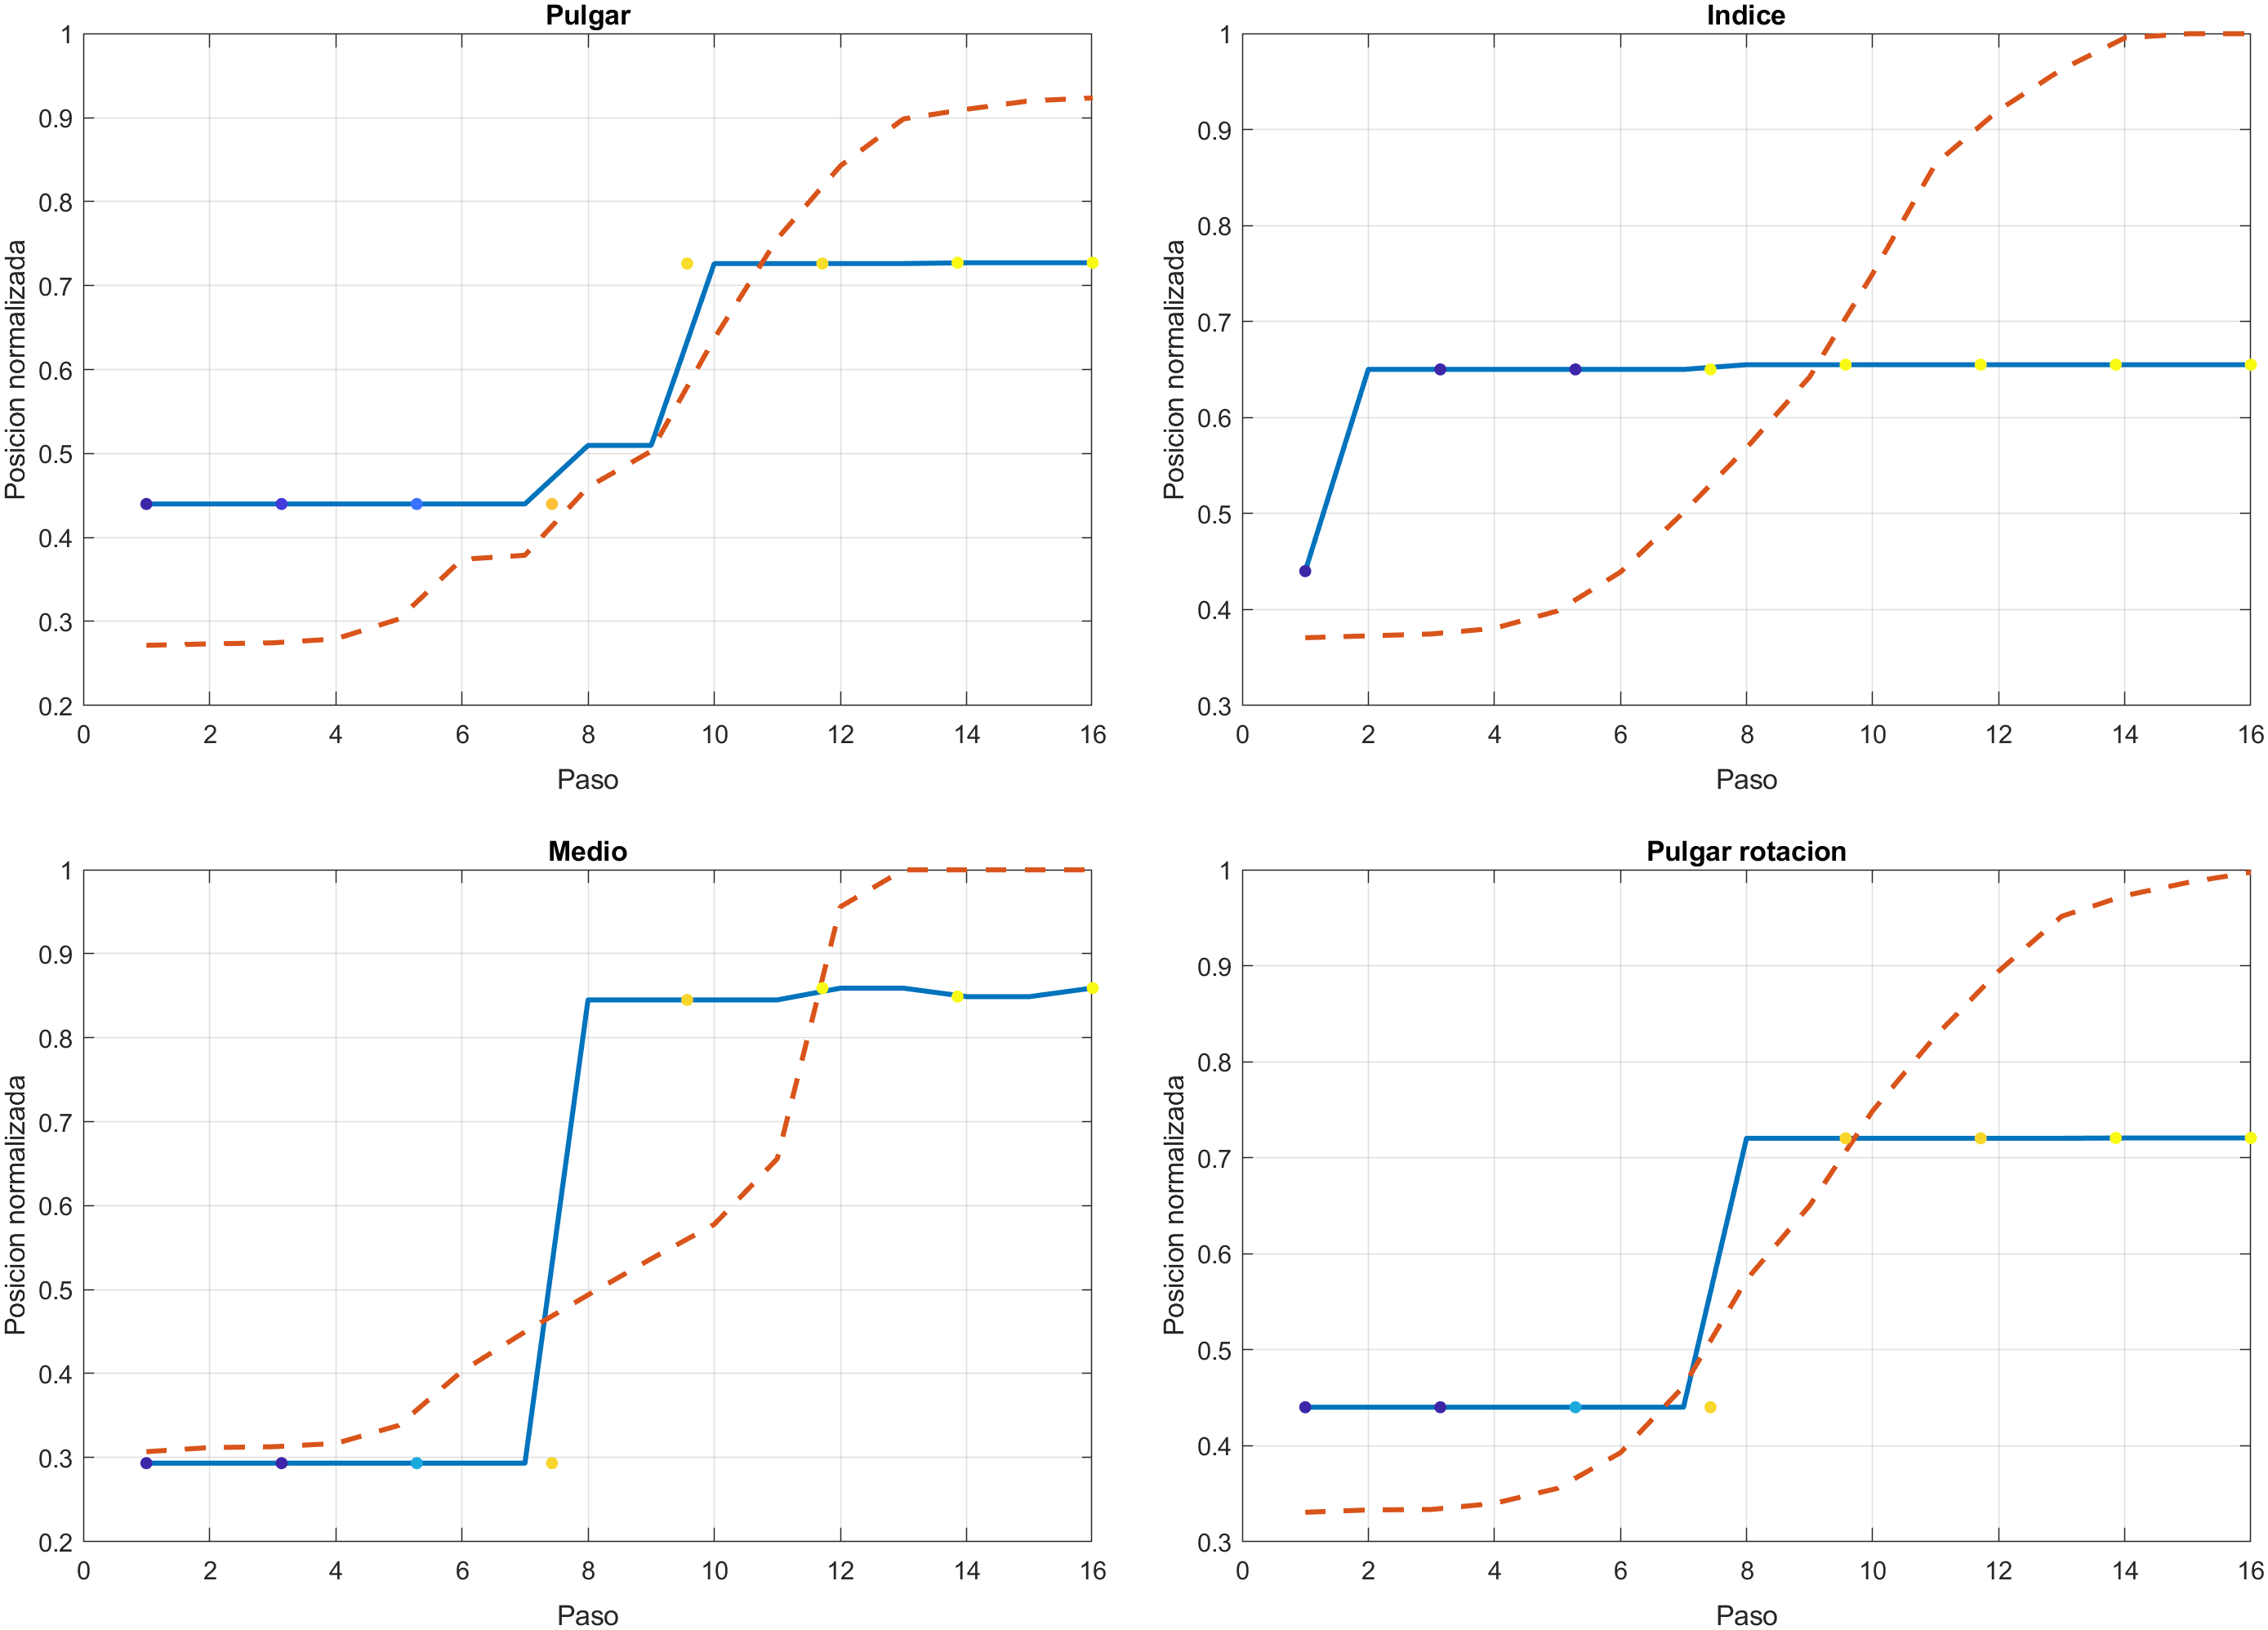
\includegraphics[width=\linewidth]{figures/longrun_residual_benchmark_visual_20260402.png}
\caption*{(b) Benchmark \texttt{Agent7250}}
\end{minipage}
\caption{Comparaci\'on visual cualitativa entre el mejor checkpoint de la corrida larga residual y el benchmark oficial.}
\label{fig:res_visuals}
\end{figure}

\section*{D\'onde conviene quedarnos y con qu\'e seguir}
La decisi\'on recomendada, despu\'es de observar estas dos corridas largas, es la siguiente:
\begin{enumerate}
    \item \textbf{Quedarnos oficialmente en \texttt{Agent7250} como benchmark.}
    \item \textbf{Mantener \texttt{seed 22} como mejor residual reproducible de referencia.}
    \item \textbf{Mantener \texttt{Agent1850} como mejor residual single-run hist\'orico.}
    \item \textbf{Cerrar las dos corridas largas como experimentos exploratorios de horizonte temporal}, \'utiles para entender meseta y desaprendizaje, pero no para promoci\'on de modelo.
\end{enumerate}

Si se decide continuar esta l\'inea a futuro, lo m\'as sensato no es empujar otra vez una sola corrida largu\'isima a ciegas. Lo m\'as razonable es:
\begin{itemize}
    \item trabajar con auditor\'ias peri\'odicas m\'as frecuentes;
    \item estudiar mejor el punto de parada;
    \item y, si se reabre la l\'inea residual, tomar como referencias activas a \texttt{Agent7250}, \texttt{seed 22} y \texttt{Agent1850}, no a las corridas largas de 50000 episodios.
\end{itemize}

\section*{Conclusi\'on general}
Las dos corridas largas cumplieron bien su funci\'on exploratoria. No demuestran que entrenar m\'as tiempo produzca un mejor agente; m\'as bien muestran algo m\'as valioso para el proyecto: tanto la base como la l\'inea residual pueden entrar en meseta y luego deteriorarse si se las empuja demasiado lejos.

Por tanto, el punto en el que conviene quedarnos ya est\'a fijado:
\begin{itemize}
    \item benchmark oficial: \texttt{Agent7250};
    \item residual reproducible de referencia: \texttt{seed 22};
    \item residual single-run hist\'orico de referencia: \texttt{Agent1850}.
\end{itemize}

Con eso, el proyecto queda mejor delimitado y mejor documentado. Las corridas largas de 50000 episodios quedan correctamente archivadas como evidencia de evoluci\'on temporal, meseta y posible desaprendizaje, que era exactamente la pregunta que se quer\'ia responder.

\end{document}
